\section{Results and Discussion}
\label{sec:result_and_discussion}

%----------------------------------------------------%
% --------- Brief Descriptive Statistics ---------%
%----------------------------------------------------%

\subsection{Brief Descriptive Statistics}
The review identified [68] articles published between 1992 and 2024. Scientific output in this area has accelerated in recent years, with the majority of papers published after 2020. As can be seen in Figure \ref{fig:scientific_productivity}, the number of published papers matching the screening criteria has increased significantly in recent years, peaking in 2024 with currently 13 publications, after a rapid growth since 2018. Thus, it is possible that the field has advanced significantly in the later years, underscoring the need for a comprehensive literature review.

\begin{figure}[H]
    \centering
    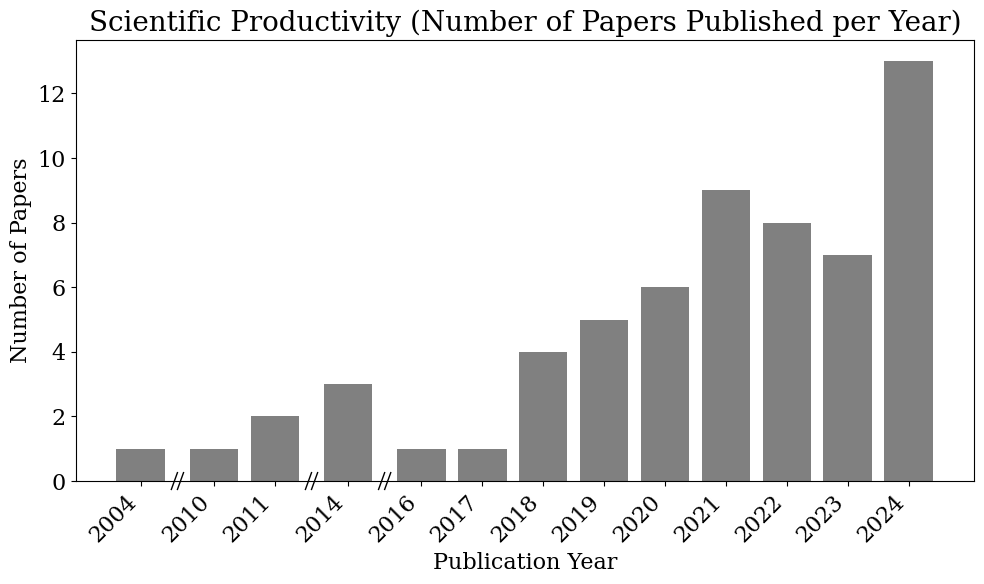
\includegraphics[width=1\linewidth]{Images/scientific_productivity.png}
    \caption{Annual distribution of papers in the field published included in the sample, illustrating the recent increase in publications}
    \label{fig:scientific_productivity}
\end{figure}

The majority of research originates from China and USA, with 17 and 8 papers contributed by authors from these countries, respectively, as shown in Figure \ref{fig:author_country_origin_per_paper}. Each country is counted only once per paper, regardless of the number of contributing authors from that country.  

\begin{figure}[H]
    \centering
    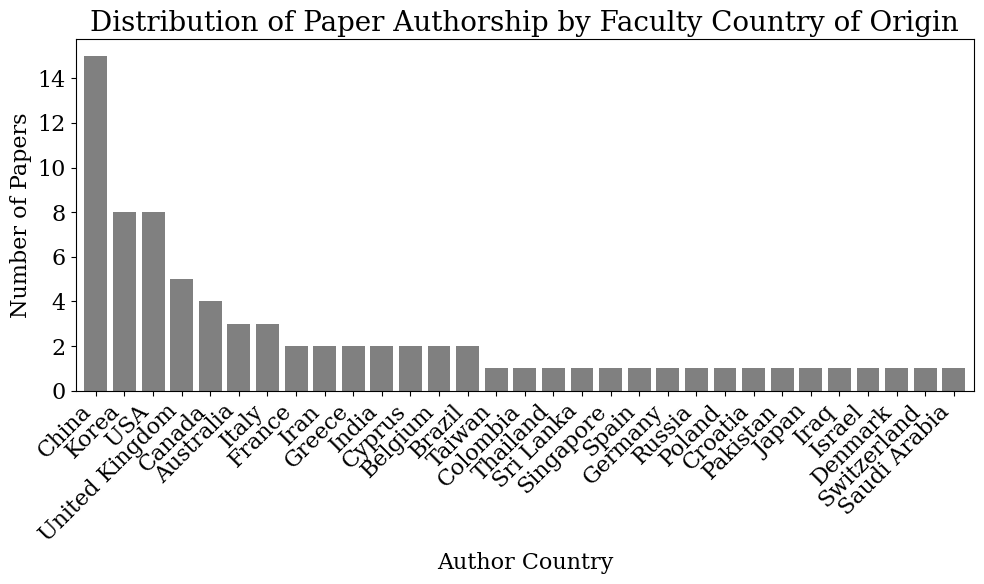
\includegraphics[width=1\linewidth]{Images/author_country_origin_per_paper.png}
    \caption{Number of articles by authors' faculty country of origin, with each country counted once per article to reflect international collaboration.}
    \label{fig:author_country_origin_per_paper}
\end{figure}

Notably, significant contributions to the field are made by authors from computer science and technical faculties, while only 20\% of authors have a background from financial, business or economics faculties, as illustrated in Figure \ref{fig:author_faculty_origin}. To capture the full scope of expertise, all authors are counted individually. 


\begin{figure}[H]
    \centering
    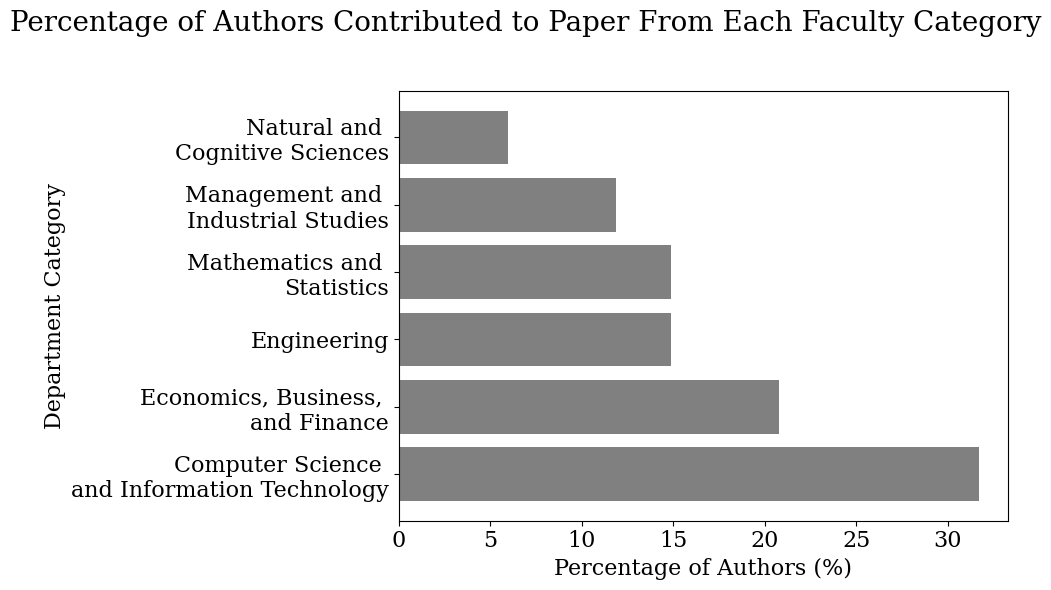
\includegraphics[width=1\linewidth]{Images/author_faculty_origin.png}
    \caption{Percentage distribution of authors by faculty category.}
    \label{fig:author_faculty_origin}
\end{figure}

In terms of journal origins, the majority of the papers from the sample were published in engineering, technical, computer science, and artificial intelligence journals or other. There are only a minor representation in finance and economics journals (15 out of 64 papers). Figure \ref{fig:num_papers_per_journal_category} shows the distribution of publications across journal categories. This distribution could suggest a potential gap in domain-specific financial research, indication a opportunity for increased financial focused journal contributions. The categorizing of journals is detailed in Appendix \ref{appendix:journal_category_mapping}. 

\begin{figure}[H]
    \centering
    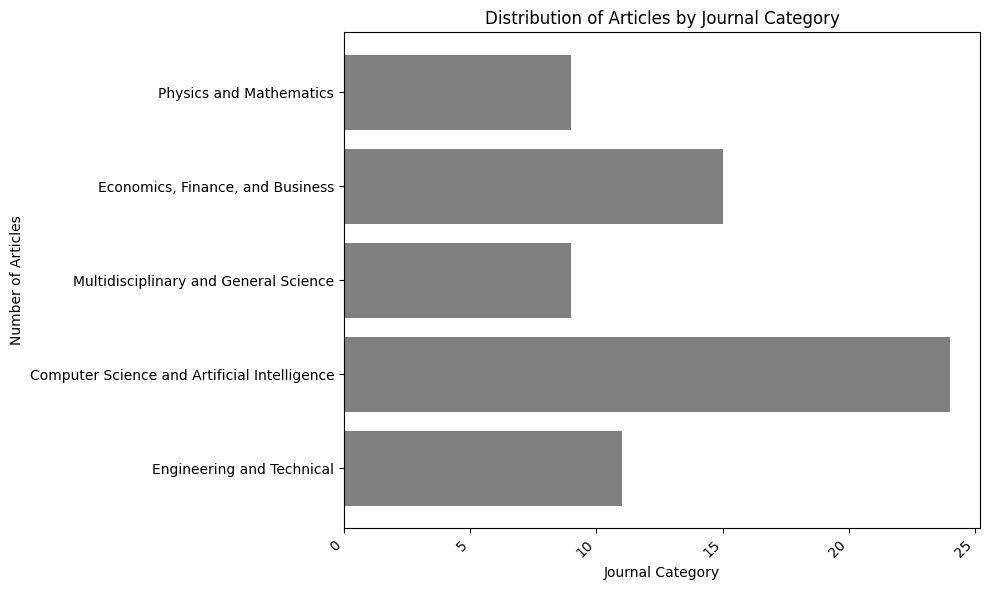
\includegraphics[width=1\linewidth]{Images/num_papers_per_journal_category.png}
    \caption{Distribution of sample papers by journal category.}
    \label{fig:num_papers_per_journal_category}
\end{figure}
The papers in the samples explores different predictive objectives within the financial domain. As shown in Figure \ref{fig:what_is_predicted}, most papers forecast asset prices, classifications or uncertainty quantification of asset prices. [CHANGE GRAPH AFTER NEW MAPPING]
\begin{figure}[H]
    \centering
    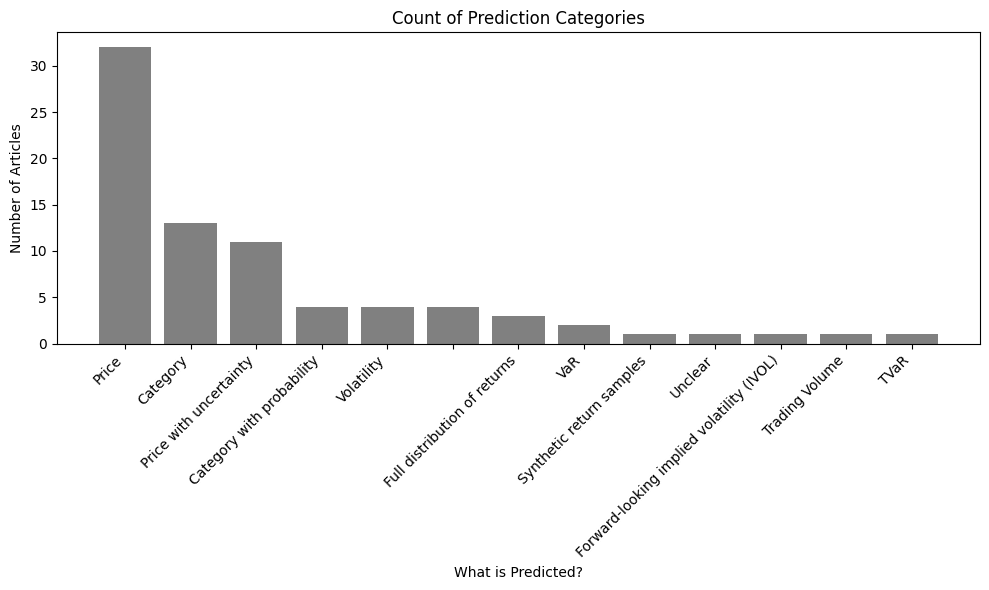
\includegraphics[width=1\linewidth]{Images/what_is_predicted.png}
    \caption{Distribution of predictive objectives in the sample papers.}
    \label{fig:what_is_predicted}
\end{figure}
Figure \ref{fig:treemap_asset_by_market} illustrates the specific financial assets and markets that are focused on and forecast in the studies. The majority of papers focus on equites, primarly stock and stock indices, but a notable number of papers also address derivatives and currencies.  
\begin{figure}[H]
    \centering
    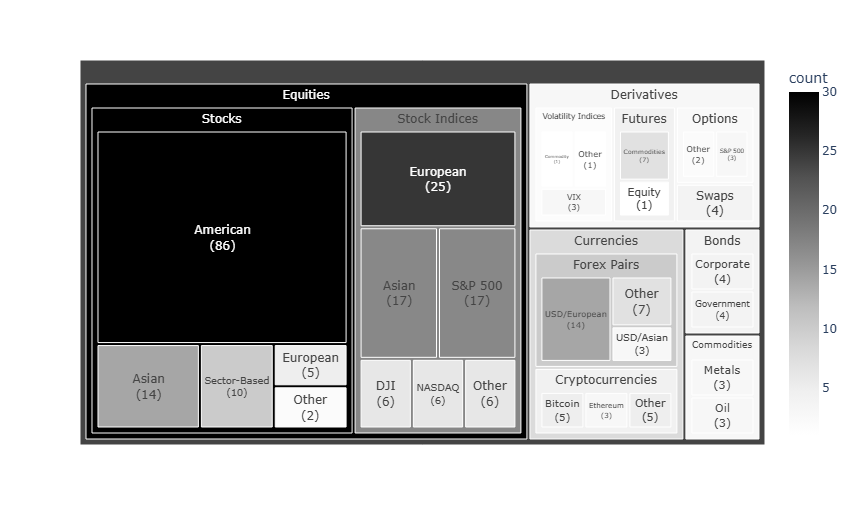
\includegraphics[width=1\linewidth]{Images/treemap_asset_by_market.png}
    \caption{Distribution of financial markets and assets targeted in the predictive models in the sample papers. }
    \label{fig:treemap_asset_by_market}
\end{figure}




%----------------------------------------------------%
% --------- Analysis by Model -----------------------%
%----------------------------------------------------%

\subsection{Analysis by Model}
\label{sec:analysis_by_model}
To give an overview of the field, we present the most predominantly used probabilistic models in the sample papers, give a description of them, depict their use, and provide an overview of how they are used to create uncertainly estimates in financial time series. Table \ref{table:model_categorization} provides an overview of probabilistic model categories created based on grouping the most commonly used model types, and specifically what model names in the papers they include. Figure \ref{fig:model_breakdown} illustrates the occurrence of each probabilistic model category, and if they are used independently or in combination with other machine learning or econometric models. Summarizing results and conclusions by model type are shown in Table \ref{table:conclusions_by_model}.

\begin{table}[H]
    \centering
    \caption[Model Categorization]{Probabilistic Model Categorization}
    \label{table:model_categorization}
    \small
    \begin{adjustbox}{width=0.5\textwidth,center}
    \begin{tabular}{p{0.2\textwidth}p{0.30\textwidth}}
        \toprule
        \textbf{Model Category} & \textbf{Models} \\
        \midrule
        Bayesian Neural Networks (BNN) & BNN, Gen-BNN, B-TABL \\
        \addlinespace
        \hdashline[0.2pt/3pt]
        \addlinespace
        Gaussian Processes (GP) & GP, GPR, G4P, GPMCH \\
        \addlinespace
        \hdashline[0.2pt/3pt]
        \addlinespace
        Variational Autoencoders (VAE) & VAE \\
        \addlinespace
        \hdashline[0.2pt/3pt]
        \addlinespace
        Hidden Markov Models (HMM) & HMM, MCHMM \\
        \addlinespace
        \hdashline[0.2pt/3pt]
        \addlinespace
        Probabilistic Recurrent Neural Network (RNN) Extensions & DeepAR, DeepARA, P-GRU, QRBiLSTM, ESVM, Bayesian LSTM, Bayes ES-LSTM \\
        \addlinespace
        \hdashline[0.2pt/3pt]
        \addlinespace
        Probabilistic Generative Adversial Networks (GAN) & CGAN, PredACGAN \\
        \addlinespace
        \hdashline[0.2pt/3pt]
        \addlinespace
        Probabilistic Neural Networks (PNN) & PNN, P FF-ANN \\
        \addlinespace
        \hdashline[0.2pt/3pt]
        \addlinespace
        Other Bayesian Methods & B-SVR, BGLM, Naïve Bayes, Bayesian Network, Facebook Prophet, BSTS \\
        \addlinespace
        \hdashline[0.2pt/3pt]
        \addlinespace
        Other Probabilistic Methods & RSMAN, PLPR, Recurrent Dictionary Learning (RDL), TV-Entropy, Gaussian Mixture Model (GMM), IMoLSO, Fitting error analysis, Probabilistic Fuzzy Logic, Leave-One-Out Cross-Conformal Predictive System (LOO-CCPS), PSVM  \\
        \addlinespace
        \addlinespace
        \bottomrule
    \end{tabular}
    \end{adjustbox}
\end{table}

\begin{figure}[H]
    \centering
    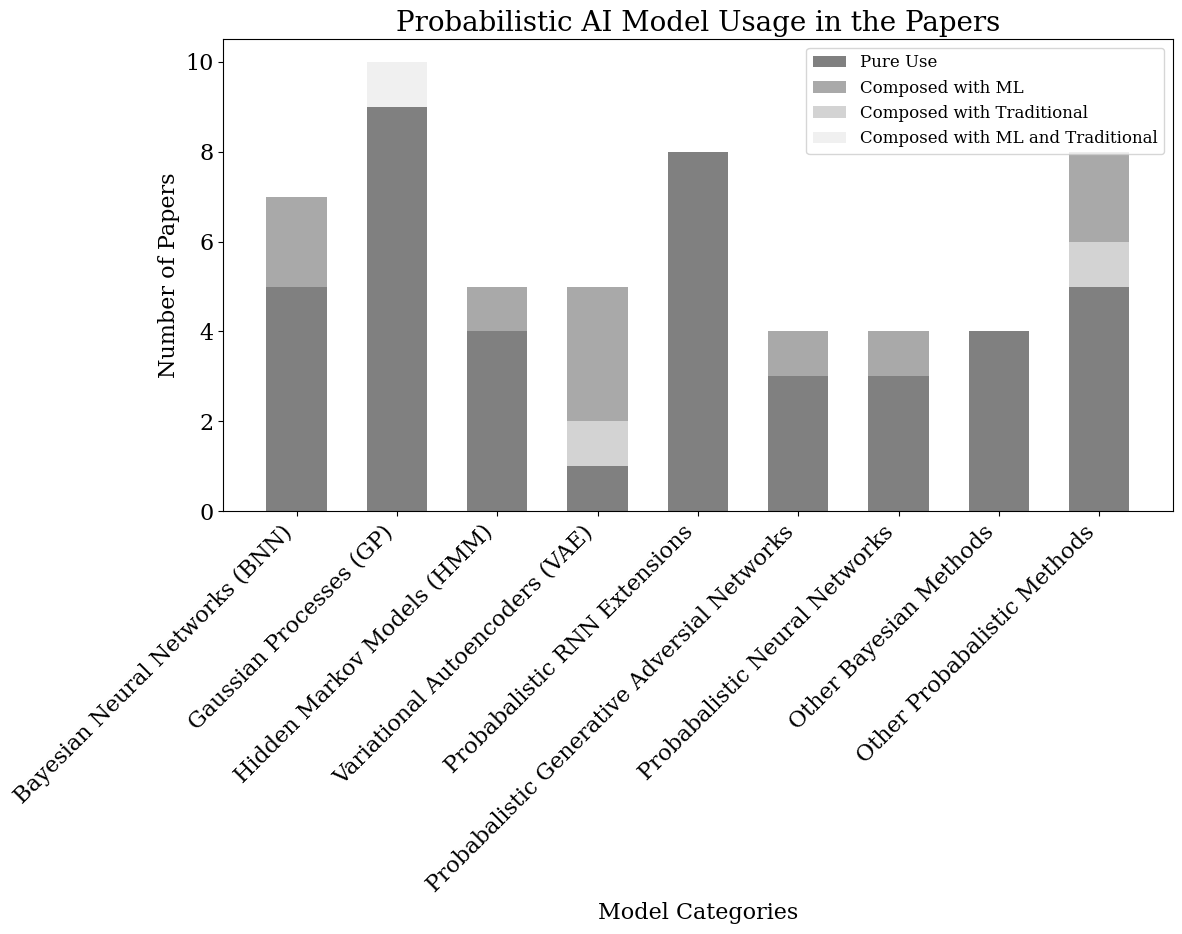
\includegraphics[width=1\linewidth]{Images/model_breakdown.png}
    \caption{Probabilistic Model Usage Breakdown}
    \label{fig:model_breakdown}
\end{figure}

%--------------------- BNN --------------------------%

\subsubsection{Bayesian Neural Networks (BNNs)}
\label{sec:bnn}

A Bayesian Neural Network (BNN) extends a traditional neural network by integrating Bayesian inference principles, allowing for the modeling of uncertainty in the network parameters \parencite{neal1995bayesian}. 
\\
\\
Conventional neural networks define a mapping from inputs $x$ to outputs $y$ using a set of trainable weights and biases $w$, represented by
\begin{equation}
    \begin{gathered}
        y = f(x;w),
    \end{gathered}
\end{equation}
where $f$ is the composition of linear transformations and non-linear activation functions across multiple layers. BNNs extend this by providing a probabilistic implementation of a standard neural network where the weights and biases are represented as random variables with probability distributions \parencite{chandra2023bayesian}, allowing the model to capture parameter uncertainty. 

Initially each weight is assigned a prior distribution
\begin{equation}
    \begin{gathered}
        p(w) = \Pi_{i} p(w_i),
    \end{gathered}
\end{equation}
where $p(w)$ represents the joint prior distribution over all weights. Combined with the likelihood of observed data $D = \{(x_n,y_n)\}_{n=1}^N$ given the weights
\begin{equation}
    \begin{gathered}    
        p(D|w) = \Pi_{n=1}^Np(y_n|x_n,w),
    \end{gathered}
\end{equation}
these form the posterior distribution over the weights using Bayes rule \parencite[p. 46]{pml1Book}
\begin{equation}
    \begin{gathered}
        p(w|D) = \frac{p(D|w)p(w)}{p(D)}.
    \end{gathered}
    \label{eq:bayes_theorem} 
\end{equation}
Predictions for new inputs $x^*$ are consequently made by integrating over the posterior distribution of the weights
\begin{equation}
    \begin{gathered}
        p(y^*|x^*,D) = \int p(y^*|x^*,w)p(w|D)dw.
    \end{gathered}
\end{equation}
By averaging over all possible weight configurations weighted by their posterior, the BNN accounts for uncertainty in parameters, resulting in a predictive distribution rather than single point estimates. This approach enables probabilistic forecasts, making them particularly suitable for uncertainty quantification \parencite{jospin2022hands}.

Both \textcite{cocco2021predictions} and \textcite{jang2018empirical} employ BNNs for cryptocurrency price predictions, primarily focusing on point estimates. \textcite{cocco2021predictions} apply a BNN with Monte Carlo approximation to predict daily Bitcoin and Ethereum prices, benchmarking against LSTM and Feed Forward Neural Networks. The BNN underperforms on Bitcoin in terms of MAPE but yields better results for Ethereum, while deployed two-stage models outperform all other. Although the authors use the BNNs outputted quantiles as prediction confidence, the authors are focused on point predictions and do not assess uncertainty. Similarly, \textcite{jang2018empirical} employ a BNN to predict Bitcoin price and volatility, using blockchain-specific data, significantly outperforming linear regression and SVR on MAPE and RSME. The authors present confidence intervals for price and volatility, which combined with the volatility estimate, could be used to assess total uncertainty. However, the probabilistic output is not leveraged to integrate these measures, nor is uncertainty explicitly evaluated as focus lie on point predictions. Notably, predictions frequently exceed the stated upper and lower bounds. 

\textcite{chandra2021bayesian} apply a BNN with Markov Chain Monte Carlo (MCMC) for multi-step stock price forecasting, benchmarking it against feed forward neural networks trained with ADAM and SGD. The BNN provide superior point estimates in terms of RSME for all stocks. The authors use the probabilistic output of the BNN to create prediction intervals as a measure of uncertainty. However, the quality or robustness of the estimate is not assessed, and evidently the actual stock price frequently fall outside the bounds for some stocks, indicating an unreliable uncertainty estimate. The authors do compare uncertainty levels during and after Covid, showing higher predicted uncertainty during the pandemic.

\textcite{soleymani2022longterm} propose a hybrid model, QuantumPath, combining a BNN with a temporal GAN to predict long-term prices for several S\&P 500 stocks. The BNN predicts the drift and volatility parameters for a Feynman-Dirac integral, which simulate stock trajectories by Monte Carlo, while the temporal GAN generates trajectories by condsidering the most probable paths. The probabilistic BNN output thus estimates the underlying probability distribution of the stock trajectories, and is therefore used implicitly as a volatility estimate. The models weighted expected values for 30-day predictions outperform models like GARCH, ARIMA and Ornstein-Uhlbeck. Even though the trajectories represent a distribution of prices, the total uncertainty is not assessed, and the BNN paramater estimates are not benchmarked against alternative methods.

\textcite{hortua2024forecasting} employ a BNN to forecast the VIX creating a hybrid architecture, combining WaveNet, a Temporal Convolutional Network (TCN) or  Transformers, with Bayesian inference techniques like the Reparametrization Trick (RT), Flipout and Multiplicative Normalizing Flows (MNF). The authors apply quantile recalibration to correct the miscalibration tendency in neural networks, addressing unreliable uncertainty estimates due to error overestimation, by aligning observed and expected data proportions within prediction intervals. assessed using Root Mean Squared Calibration Eroor (RMSCE). The models using MNF demonstrate the most reliable predictions, and generally superior short-term point predictions, outperforming traditional ARIMA. 

\textcite{magris2023bayesian} introduce a Bayesian Temporal Augmented Bilinear Network (B-TABL) for forecasting and classifying mid-price changes in Limit Order Books (LOB). Employing a Variational Online Gauss-Newton (VOGN) method for Bayesian inference, the model yield better calibrated class probabilities than approaches like Monte Carlo Dropout. Expected Calibration Error (ECE) and Expected Calibration Distance (ECD) are used to evaluate how well predicted probabilities align with actual observed frequencies, assessing model reliability in uncertainty estimation. The BNN framework provide predictive distributions for class probabilities, offering an uncertainty measure the authors interpret as confidence. While VOGN optimizer for B-TABL does not clearly outperform ADAM on standard classification metrics, the authors argue that the model deliver more meaningful classifications due to superior calibration scores. 


%--------------------- GPR ------------%

\subsubsection{Gaussian Process Regression (GPR)}
Gaussian Processes Regression (GPR) is a probabilistic, non-parametric Bayesian model used for regression tasks. Much of the modern framework for Gaussian Process Regression in machine learning was formalized by \textcite{rasmussen_williams_2006}. Gaussian process is used to perform inference over functions, defining a distribution over possible functions $f(x)$  that fit the given data. Formally, a Gaussian Process (GP)  is defined as: 
\begin{equation}
f(x) \sim \mathcal{GP}(m(x), k(x, x'))
\end{equation}
where $m(x)$ is the mean function $\mathbb{E}(f)$, and $k(x, x')$ is the covariance function, also known as kernel defining how function values at point $x$ and $ x'$ effect each other:
\begin{equation}
k(x, x')=Cov(f(x),f(x'))
\end{equation}
Based on the posterior distribution, Bayesian inference (\ref{eq:bayes_theorem}) is applied to determine the most likely function $f$ that fit the data   making it possible to make new prediction as new data is observed \parencite{rasmussen_williams_2006}. Since GPR provides  a predictive mean $\mathbb{E}(f_*)$ and a predictive variance $Var(f_*)$ , it allows for producing both predictions in addition to uncertainty estimates and confidence intervals for each prediction. GPR is therefore inherently probabilistic since it instead of only providing a single point estimate provides a distribution over predictions.  The probabilistic output consequently make GPR highly useful for modeling uncertainty in financial time series, where the degree of uncertainty often is more important than the prediction itself. 

There are 11 papers in  total that use GPR. Mainly used independently, only X papers has combined it with other ML models. 

\textcite{Suphawan2022gpr} employed GPR to tackle the non-linear and non-stationary nature of the market when forecasting the Stock Exchange of Thailand (SET), and tested across different periods including the Covid-19 pandemic. The model was compared to ANN and RNN and demonstrated superior prediction accuracy on traditional error measures (RMSE, MAE, MAPE, NSE). The model allowed for providing confidence interval of the prediction results witch the authors colcudes makes GPR advatagous compared to ANN and RNN models. 

In \textcite{Wang2021gpr} a multi-scale nonlinear ensemble model incorporates GPR to predict stock indices for S\&P 500, Dow Jones and NASDAQ. The ensemble model use Variational Mode Decomposition (VDM) and an Auto-Encoder (AE) for feature extraction, and a two-step deep learning setup with RNN and LSTM. GPR plays a critical role in the final stage to create interval prediction and uncertainty estimates. The model is benchmark against a regular GPR and other machine learning models such as ANN, RNN and LSTM, displaying improvements in MAPE, MSE, RMSE, MAE and SSE for point predictions. In addition the interval prediction are asses on coverage probability metrics like Mean width percentage (MWP), Mean coverage (MC) and Prediction interval coverage probability (PICP) which shows better results than GPR alone. In another paper by the same authors, \textcite{Wang2021gprensemble} presents an alternative esamble (SSA-EWSVM-RNN-GPR) for stock index forecasting using Singular spectrum analysis (SSA) and Enhanced weighted support vector machine (EWSVM) for interval prediction, which is then further process by an RNN before GPR is used to provide interval forecasts. MWP and CP were used to validate the GPR-based interval forecast and the model showed improved point accuracy forecasting and uncertainty estimate compared to eight GPR benchmark models.  

\textcite{Li2024gpr} integrated a GPR model into a graph-aware portfolio selection model with Generalized Gaussian Distribution (GGD) likelihood capturing both return mean and variance. The GPR model showed improvements compared to some traditional mean-variance methods, but is outperformed by amongst other Uniform Constant Rebalanced Portfolio (UCRP). 

\textcite{Platanios2014gpr} adopted a GPR model int a Gaussian Process Mixture Conditional Heteroscedasticity (GPMCH) model to forecast price and financial volatility for currency exchange rates and global large-cap equity indices.  It combines GPR with a mixture model to capture volatility clustering and handle the non-linear dependency, presenting a viable alterative to traditional GARCH models. The authors applies a Pitman-Yor process to better capture skewed and tail heavy data distributions, and showed that their GPMCH outperformed GARCH in volatility predictions. 

Estimation of portfolio tail risk, specifically VaR and TVaR, has seen accuracy improvement with GPR models as demonstrated by \textcite{Risk2018gpr}. The models spatial modeling enabled efficient risk estimations across simulated economic scenarios with Monte Carlo simulations. Bias and variance in the risk estimates was reduced compared to traditional nested simulations and methods. The author use the model to distinguish between epistemic and aleatoric uncertainty. In one of the advanced models the authors present, they use heteroskedastic GP (hetGP), witch allowed for handling scenarios of varying levels of noise more effectively, further enhancing the uncertainty estimates. 

The last studies in the sample utilizing GPR;  \textcite{Papaioannou2022gpr}, \textcite{Zmuk2020gpr}, \textcite{Park2014gpr}, and ~\textcite{DeSpiegeleer2018gpr} apply GPR for price prediction in financial time series and \textcite{Hocht2024gpr} predict forward-looking implied volatility (IVOL), generally demonstrate competitive performance against traditional models. However, these works focus primarily on point predictions without assessing the probabilistic outputs of the GPR model or quantifying prediction uncertainty.




%--------------------- VAE --------------------------%


\subsubsection{Variational Autoencoders (VAEs)}
Variational Autoencoders (VAEs) are generative models that combine principles from deep learning and variational inference to learn probabilistic representations of data. Introduced by \textcite{kingma2013auto} as Auto-Encoding Variational Bayes, the model architecture distinguishes itself from traditional autoencoders by utilizing stochastic elements in the two main components: the encoding and decoding processes. 
\\
\\The encoder maps input vector data $x$ to a latent space $z$, producing the parameters (mean and variance) of a probability distribution $q_\phi(z|x)$ over the latent variables, where $\phi$ denotes the parameters of the encoder network. The decoder subsequently reconstructs the original input data from this latent representation by mapping samples $z \sim q_\phi(z|x)$ through $p_{\theta}(x|z)$ aiming to model the true distribution
\begin{equation}
    \begin{gathered}
        p_\theta(x) = \int p_\theta(x|z)p(z)dz,
    \end{gathered}
\end{equation}
where the decoder is parameterized by $\theta$. However, due to intractable computation of the exact posterior $p_{\theta}(z|x) = \frac{p_{\theta}(x|z) p_{\theta}(z)}{p_{\theta}(x)}$, variational inference over the latent variables is employed to approximate it with $q_\phi(z|x)$ \parencite{kingma2013auto}. As the encoder outputs a distribution over the latent variables, uncertainty can be captured in the latent representation by drawing multiple samples. These samples can then be propagated through the decoder, ultimately resulting in a distribution of reconstructed outputs. 


Only one article in the sample uses a VAE independently. \textcite{arian2022encoded} propose Encoded VaR, directly applying VAE to estimate VaR by generating synthetic market scenarios from historical cross-sectional stock returns of the S\&P 500, LSE and FSE. The VAE learns the latent structure of the financial return distributions without relying on parametric assumptions or predefined joint distributions, and in turn generating samples of synthetic returns to be interpreted as potential future outcomes. The VAE architecture allows generation of arbitrarily many samples, allowing the reconstruction a theoretical underlying distribution for VaR calculation. The authors claim to enhance the signal-to-noise ratio present in financial data, and benchmark against traditional GARCH models. While the model shows competitive results for specific loss functions like Lopez' method \parencite{lopez1998methods}, GARCH extensions (CaViaR-GARCH and EVT-GARCH) generally perform equally well and yield statistically significant p-values across all adequacy tests, in contrast to the Encoded VaR. 

Of the papers utilizing VAEs in combination with other models, several use it as a probabilistic input to another model and do not directly infer uncertainty estimates from the probabilistic output of the VAE.  
\textcite{caprioli2023quantifying} extend the use of VAEs for risk management to assess credit portfolio sensitivity to asset correlations. The VAE is used to generate synthetic correlation matrices, simulating various market conditions, used as input in a multi-factor Vasciek model with Monte Carlo simulation to examine how shifts in correlations affect VaR. \textcite{choudhury2020enhancing} use VAEs as a pre-processing tool to denoise NASDAQ stock financial time series before using a stacked LSTM autoencoder to make point predictions. The authors report superior results in point predictions compared to other machine learning models like, but do not assess uncertainty in their forecasts.  \textcite{tang2024period} also uses VAEs for denoising financial time data by extracting latent representations. The model is combined with a transformer (LPAST), and is used for long-term multi-step point predictions of different financial times series. The proposed method outperforms compared machine learning models in point predictions, but again the probabilistic outputs of the VAE are not directly utilized for distributional forecasts or for uncertainty quantification. \textcite{li2020multivariate} combine a multimodal VAE with a LSTM architecture to predict agriculture commodity futures. The VAE is used to extract high-level features and reduce noise for input data in the LSTM, and probabilistic output is not used specifically in predictions. Their proposed model outperforms traditional econometric models like ARIMA, and other machine learning benchmarks like CNNs. 

\textcite{xing2019sentiment} propose an innovative approach by combining VAEs with a RNN to forecast stock volatility. Their model, Sentiment-Aware Volatility Forecasting (SAVING), integrates social media sentiment data to jointly model stock price movements and the sentiment that influences them. This interaction is captured through the VAE's latent variables, from which marginal joint probabilities are inferred. Benchmarked against econometric models GARCH, EGARCH and TARCH using negative log-likelihood, the SAVING model demonstrate superior performance.

%--------------------- HMMs --------------------------%

\subsubsection{Hidden Markov Models (HMMs)}
Hidden Markov Models (HMMs) are probabilistic models used to analyze sequential data where there exists underlying unobservable structures \parencite{rabiner1986introduction}, building on foundational theory of Markov chains and stochastic processes. In finance, HMMs can therefore be applied to model time series where market states, such as bull or bear markets, periods of low or high volatility, or other economic regimes, are not directly observable. 

The classic HMM consists of a finite set of hidden states $S = \{s_1, s_2, ... s_N\}$ and a corresponding set of observable outputs $O = \{o_1, o_2, ... o_T\}$. The model is defined by an initial probability distribution $\pi_i = P(q_1 = s_i)$, state transition probabilities $a_{ij} = P(q_{t+1} = s_j|q_t = s_i)$ and the emission probabilities specifying the likelihood of observations given system state $b_j(o_t) = P(o_t|q_t=s_j)$. Consequently, HMMs are capable of producing distributional forecasts by utilizing the predictive probability distribution of future observations
\begin{equation}
        P(o_{T+1}|O) = \sum_{i=1}^{N}P(o_{T+1}|q_{T+1} = s_i)P(q_{T+1} = s_i | O).
\end{equation}
The probabilistic modeling of both hidden states and observations allow for the computation of confidence intervals and prediction reliability, thereby facilitating uncertainty estimation of predictions. 

Two articles in the final sample use HMMs to address multi-factor dependencies in financial time series forecasting. \textcite{li2010stochastic} propose a stochastic HMM for forecasting fuzzy time series data, modeling the Taiwan Weighted Stock Index as the hidden states and the New Taiwan dollar against the U.S. dollar as the observable state. While the model performs better compared to a standard HMM implementation in forecasting accuracy, it is not evaluated against any other models. Additionally, they focus solely on point predictions, without assessing the probabilistic output of their model. \textcite{cao2019multi} extend the multi-factor dependency approach by developing a Multi-Layer Coupled HMM (MCHMM). Unlike \textcite{li2010stochastic} who address dependencies within a single market, \textcite{cao2019multi} capture interactions both within and between markets, specifically between stock and currency markets across different countries. The authors experiment predicting categorical trends of German and Dutch stock markets, reporting better accuracy than traditional models like ARIMA and logistic regression. However, similar to \textcite{li2010stochastic}, they  do not assess uncertainty in predictions that can be derived from the probabilistic output of the model. 

\textcite{sher2023exploiting} also focus on forecasting categorical return trends, applying HMM alongside several other models to forecast movements in individual technology stocks. Although the details around their specific model implementation are limited, the authors report superior performance from the HMM compared to ARIMA, LSTM and several booster models. The probabilistic output of HMM is leveraged to assess the likelihood of future stock price movement, but like the previous studies, uncertainty assessment is not addressed. 

\textcite{zhang2019high} extend the HMM to a second-order model, capturing both short-term and long-term dependencies for predicting next-day categorical trends in stock indices. In their higher order approach, the observation depends not only on the current state, but also on the previous $m-1$ hidden states. While the authors do not directly use the probabilistic distribution output to assess uncertainty, they suggest that the higher-order HMM has lower risk then the first-order model, supported by improved Sharpe ratios and reduced maximum drawdown in their trading strategy experiment. Additionally, the second-order HMM deliver better predictive performance compared to the first-order HMM.

Similarly, \textcite{su2022hmm} applies the second-order HMM model to predict prices and directions of the Hang Seng Index (HSI). Even though their model is capable of producing distributional forecasts, the authors focus exclusively on point predictions and do not assess uncertainty of any kind. When compared to models like NA-GARCH, CNN-BiLSTM-AM and AHMMAS, the second-order HMM showcases superior performance. 


%--------------------- Prob RNN extensions --------------------------%


\subsubsection{Probabilistic RNN Extensions}
\label{sec:prob_rnn}

Probabilistic extensions of Recurrent Neural Networks (RNNs) refer to models augmenting standard RNN implantations with stochastic components, enabling them to generate probabilistic forecasts. RNNs are neural networks designed to handle sequential data by maintaining hidden states that capture information about previous inputs to shape subsequent behavior \parencite{Elman1990Finding}, making them suitable for financial time series analysis. In a standard RNN the hidden state$h_t$ at time step $t$ is updated based on the current input $x_t$ and the previous hidden state $h_{t-1}$:
\begin{equation}
    \begin{gathered}
        h_t = \phi(W_{xh}x_t + W_{hh}h_{t-1} + b_h)
    \end{gathered}
\end{equation}
where $\phi$ is an activation function, $W_{xh}$ and $W_{hh}$ are weight matrices and $b_h$ is a bias vector. 

Standard RNNs suffer from the exploding and vanishing gradient problems \parencite{Pascanu2013Difficulty}, which hinder long-term dependencies and make training difficult. To address this issue, advanced architectures like Long Short-Term Memory (LSTM) networks \parencite{Hochreiter1997LSTM} and Gated Recurrent Units (GRU) \parencite{Cho2014Learning} have been introduced, incorporating gating mechanisms to control the information flow. 

Several articles apply Bayesian methods within RNN implementations, placing prior distribution over the network weights to estimate the posterior distribution (Equation \ref{eq:bayes_theorem}). \textcite{Hassan2024Bitcoin} utilize a Bayesian LSTM with MC dropout at inference, optimized with ADAM, to generate a distributional forecast of Bitcoin prices. The model outperforms non-Bayesian LSTMs in RMSE, $R^2$ and MAPE for point predictions, and the Bayesian approach facilitate model uncertainty quantification. The author argue that model uncertainty is accurately estimated, as it increases with prediction distance from actual data, but no other assessment measure of the quality of the uncertainty estimate is utilized. Similarly, \textcite{Dixon2022Industrial} incorporate exponential smoothing within a Bayesian RNN, smoothing hidden states to capture long-term dependencies in IBM stock predictions. The model provide more accurate forecasts compared to a standard LSTM and GRU implementation, with better coverage of confidence intervals across various predictive horizons. This improvement is presented as evidence of superior uncertainty estimation, though no distinction between model uncertainty and aleatoric uncertainty is made.

\textcite{Parker2021BayesianHeteroskedastic} present a Bayesian general heteroskedacity model (GBHM) within an RNN framework to predict Dow Jones index volatility. Compared to a GARCH implementation, the model achieves superior log predictive scores. Additionally, the authors report more accurate uncertainty measured by coverage, with GARCH yielding an inflated 100\% coverage for the 50\% prediction interval, while the model attains nearly optimal 50\%. Previous research has shown that GARCH generally produces reliable coverage probabilities when modeling stock indices [kilde], so this result raises questions about whether the GARCH model they have benchmarked against is misspecified.

\textcite{Golnari2024Cryptocurrency} introduce a probabilistic GRU model incorporating Bayesian inference to treat network weights as probabilistic, enabling distributional forecasts
 for crypto price predictions. The model outperforms traditional LSTM and GRU implementations in MAPE and $R^2$ of point predictions. The authors use the standard deviation of the forecast distributions as a measure of prediction uncertainty, but do not further assess it's reliability or distinguish uncertainty types.  

\textcite{Wang2024GoldForecasting} employ Quantile Regression (QR) within a Bi-Directional LSTM model to produce probabilistic range predictions for gold prices, incorporating several macroeconomic factors. The QR-BiLSTM predicts multiple quantiles of the future price distribution, capturing price fluctuations and is used as a measure of uncertainty. The authors assess the total uncertainty of the predicted distributions, without separating model and underlying uncertainty, using the Average Internal Score (AIS), which balances interval width and accuracy. This evaluation demonstrate that their model outperform other LSTM and GRU benchmarks. 

Three articles in the sample employ the DeepAR model \parencite{Salinas2019DeepAR}, an autoregressive RNN-based model that generate parameters of a predefined probability distribution at each time step. \textcite{Fatouros2023DeepVaR} apply DeepAR to forecast VaR for a forex portfolio, comparing it to GARCH and other models using Christoffer's and Dynamic Quantile tests for adequacy. Their results are promising as the adequacy tests are passed, with superior accuracy in most loss functions. \textcite{Almeida2024RiskForecasting} use DeepAR to forecast VaR and ES for crypto liquidity pool portfolios, reporting superior accuracy in ES prediction over GARCH. However, without any adequacy tests, interpretation of results is unvalid. \textcite{Li2024DeepAR} extend DeepAR with an attention mechanism (DeepARA) for stock price forecasting in the Chinese market, achieving superior MAPE in point predictions compared to other neural networks. The authors assess uncertainty by analyzing the entropy of the predicted price distributions concluding that the model provide good estimates, but lack comparative uncertainty evaluation, as no alternative models considered provided comparable distributions.  

%---------------------  P GANs --------------------------%


\subsubsection{Probabilistic Generative Adversarial Networks}
Generative Adversarial Networks (GANs) are a class of deep learning models that was introduced by \textcite{goodfellow2014gan}, providing a framework for estimating generative models though adversarial process \parencite{goodfellow2014gan}. GANs consist of two neural networks, a generator $G$ and a discriminator $D$ that are trained in a two-player competitive minimax game.
The generator produce synthetic data that aims be as close to real data as possible, while the discriminator ties to distinguish between synthetic and real data samples. Both network iteratively try to improve. 

The probabilistic capabilities of GANs comes from the generators ability to map random noise $p_z(z)$, like for example Gaussian, to a probability distribution of outputs similar to the real data distribution $p_{\text{data}}(x)$ enabling it it capture the uncertainty in real-world-data. The objective can formally be formulated as: 
\begin{equation}
\min_{G} \max_{D}  \mathbb{E}_{x \sim p_{\text{data}}(x)}[\log D(x)] + \mathbb{E}_{z \sim p_z(z)}[\log (1 - D(G(z)))]
\end{equation} 

Four articles in the sample used GANs in their financial forecasting. For example, \textcite{lee2021estimation} proposed a modified conditional GAN (cGAN-UC) as probabilistic model to forecast price of NASDAQ-100 Future Index with uncertainty. The authors used the generator to predict rather than for sample generation to be used as a probabilistic predictive neural network. The cGAN model outperformed traditional deterministic models such as Artificial Neural Networks (ANNs), Random Forest, Ridge and Lasso regression and probabilistic models like Bayesian Neural Networks (BNNs) for both point accuracy and uncertainty estimation especially in noisy data due to the benefits of adversarial training. 

\textcite{vuletic2024finGAN} introduced a specialized GAN model (Fin-GAN) for one-step-ahead probabilistic prediction of stock and stock indices price with uncertainty. The model uses a cGAN architecture with an economics-driven loss function, to enhance Sharpe Ratio and integrate risk directly in the model. The model outputs a full conditional probability distribution of returns witch allows it to estimate the financial uncertainty. The Fin-GAN model claims to outperform and achieve higher Sharpe Ratio compared to traditional time-series modes such as ARIMA and LSTM, and allows for uncertainty informed portfolio allocation due to its probabilistic outputs. However, the paper does not compare the uncertainty estimation against other probabilistic or ML models. 

For portfolio optimization, \textcite{kim2023portfolio} applies a predictive auxiliary classifier GAN (PredACGAN) on S\&P 500 and NASDAQ 100 stocks. The generator forecast future returns based on historical data and produce distributions reflecting prediction uncertainty. The authors construct a portfolio based on the predictions, where they combine the expected return with the distribution's entropy as a risk measure to maximize risk-adjusted returns. The PredACGAN portfolio resulted in higher Sharpe Ratio and lower maximum drawdowns in comparison to traditional risk-agnostic portfolios and other ML models (e.g. Ridge classifiers and gradient boosting).

\textcite{salama2024gan} applies a similar approach using a cGAN model but aims to increase performance by integrating a spotted hyena optimization algorithm with a GAN for time series forecasting (SHOAGAI-TSF) technique. The Spotted Hyena Optimization Algorithm (SHOA) optimize the models hyperparameters to enhance prediction accuracy. The integration improves Mean Absolute Error (MAE) and Mean Squared Error (MSE) performance compared to other GAN-based model, however the paper even though the model provides full probabilistic distribution, the paper does not use it to asses uncertainty but focus on improving prediction accuracy. 


%--------------------- PNNs --------------------------%

\subsubsection{Probabilistic Neural Networks (PNNs)}
Probabilistic Neural Networks (PNNs) is a type of feedforward neural network with four layers leveraging statistical principles for mainly for classification tasks first introduced by \textcite{Specht1990pnn}, that builds on Bayesian decision theory in order to estimate full probability distribution for the cases given the input \parencite{Specht1990pnn}. PNNs are inherently probabilistic as they utilize probability density functions (PDF) to create output based on posterior probabilities making it possible for confidence assessment of the classifications. The class-conditional probability for an input $x$ is given by:

\begin{equation}
P(x \mid C_i) = \frac{1}{N_i} \sum_{j=1}^{N_i} \exp \left( -\frac{\| x - x_j \|^2}{2\sigma^2} \right)
\end{equation}
where $x_j$ are samples from $C_i$, $N_i$ number of samples in class $C_i$ and $\sigma$ is a smoothing factor. 
The probabilistic structure makes it possible for dynamic probability estimations based on new data and suitable for real-time assessment and decision-making with confidence levels for classification. 

Four papers in the sample apply PNNs.
\textcite{Thawornwong2004pnn} utilized a PNN model to predicting the directions of future
excess stock return for S\&P 500 stock portfolio, where they investigate adaptive selection of economic variables for prediction by using recent relevant variables. The model demonstrates an ability to outperform traditional models such as linear regression, random walk model and neural network with constant variables. However, the model focus on directional accuracy and risk-adjusted profits to provide an alternative to the buy-and-hold strategy with reduced risk and increased profitability, rather than uncertainty quantification assessment.  

\textcite{Chandrasekara2019pnn} enhance the traditional PNN using multivariate t-distribution instead of Gaussian assumption. The authors explore this approach to improve the traditional PNNs by integrating multivariate distribution to better capture the relationship and the joint distribution of input variables. In addition they proposed a solution for addressing multi-class imbalance to prevent biased directional predictions. The model was tested on three stock market indices (AORD, GSPC, API). The proposed model with scaled t-distribution and  the multi-class undersampling based bagging (MCUB) ensemble method showed better performance and accuracy than standard PNN models independently and together in directional forecast, although the paper does not explicitly focus on uncertainty quantification.  

\textcite{Maniatopoulos2022pnn} propose a probabilistic feed-forward artificial network (Probabilistic FF-ANN) to predict category with probability for company stocks in US Down Jones. The proposed solution builds on the PNN framework with probabilistic recovery to enhance predictive accuracy across time horizons integrated. The authors claim the Probabilistic FF-ANN outperforms CNN, FFNN, LSTM and GAN models, and are able to give 60\% future movements accuracy and a reported 60\% annual return on investment. 

\textcite{Lahmiri2024pnn} compares a PNN with a Back-Propagation Neural Networks that is optimized using 
Genetic algorithms (GA-BPNN) for prediction daily trends in tech stocks and the NYSE index. Their results show that GA-BPNN outperforms the traditional PNN in accuracy. Although the study show that PNN effectively leverage the probabilistic output for classification, it does not assess uncertainty quality.  

%--------------------- Other Bayesian methods -----------------------%

\subsubsection{Other Bayesian methods}
Other Bayesian Methods refer to models that apply Bayesian techniques and are able to construct probability distributions to quantify uncertainty, without utilizing Bayesian inference in Neural network architectures. Rather than delving into the technical implementations of each model, we will focus on summarizing the key results they achieve. 

\textcite{Malagrino2018Forecasting} utilize a Bayesian network to predict the directional movements of the Brazilian iBOVESPA index by incorporating dependencies among multiple global stock indices, achieving competative accuracy with comparable literature. Although the Bayesian network model generally provide well-calibrated probabilities for classification, the authors classify binary without explicitly quantifying uncertainty in classification outcomes. Similarly, \textcite{Raúl_PlazaCasado_PradoRomán_2021} apply a Bayesian network to forecast IBEX index trends, incorporating investor sentiment to enhance model performance. Here, the authors interpret the classification probabilities as trust levels that indicate degrees of uncertainty, and develop a trading system shown to systematically outperform the market.

\textcite{Grudniewicz2023Application} evaluate a Bayesian Generalized Linear Model (BGLM) alongside traditional and machine learning models for classifying stock movements to generate trading signals across various indices for algorithmic trading. Their findings indicate that algorithmic trading outperformed passive strategies, with the BGLM was among the most accurate models. However, the probabilistic output of the BGLM is not use to assess uncertainty, nor integrated into the trading strategies. 

A distinct application is proposed by \textcite{Law2017Practical}, using a Bayesian Support Vector Regression (B-SVR) for price prediction and prediction uncertainty estimates for various financial time series classes, including equity indices, commodity futures and bond yields. The Bayesian framework optimize model parameters, and the complete model produce interval predictions. The authors evaluate the uncertainty estimate quality by examining the correlation between prediction uncertainty and actual errors using the Coefficient of Variation (CoV), classifying predictions as reliable or unreliable based on a continuously calibrated threshold value, excluding unreliable predictions. The model is not benchmarked against traditional or ML models. 

%--------------------- Other probabilistic methods --------------------------%

\subsubsection{Other Probabilistic Methods}
Other Probabilistic models refer to methods capable of producing probabilistic forecasts, but do not fit easily in any of the aforementioned categories. We will present a short summary of some of the 11 articles in the category and what results they report, but will not delve into technicalities in this section. Descriptions of the rest can be found in Table \ref{table:...} 

\textcite{Daniali2021} employ a Deep Convolutional Neural Network (DCNN) to forecast the VIX, integrating a conditional variance model in the final layer to jointly predict mean and variance. The variance is embedded within the probability-based loss function as a way to reduce uncertainty. Compared to a standard DCNN, the model demonstrated reduced error in point predictions. 

\textcite{Tian2023} also forecast volatility indices using a Clockwork RNN optimized with a Cuckoo-Search-enhanced multi-objective grey wolf optimizer, employing empirical mode decomposition to capture both linear and nonlinear trends. The model produces deterministic and probabilistic forecasts, with uncertainty quantified and distinguished using PICP, PINAW, and Winkler score. It demonstrates superior accuracy and stability across case studies, including the VIX, crude oil ETF volatility index (COEVI), and the 10-year U.S. treasury note volatility index (TYVIX).

\textcite{Horenko2020} propose a multivariate nonparametric regime-switching model (TV-Entropy) based on the maximum entropy principle, applying it to forecast stock indices and estimate VaR. Compared to GARCH, TV-Entropy achieves superior Bayesian Information Criterion (BIC) scores, and better calibrated unconditional coverage on 95 and 99\% confidence intervals. 

\textcite{Sharma2021} introduce Recurrent Dictionary Learning (RDL), which incorporates the Kalman filter with smoothing algorithms to generate distributional forecasts for stocks. The model outperforms LSTM, CNN, and ARIMA in both point forecasts and next-day trend classification, while no explicit assessment of uncertainty is conducted.

\textcite{Guo2022} forecast non-ferrous metal futures using a combined kernel extreme learning machine (CKELM) optimized by a multi-objective lion swarm algorithm. The model generates prediction evaluated by PICP, PINAW and AIS, outperforming other ML benchmarks like standard extreme learning machines and BPNNs, as well as providing more accurate point predictions.

\cite{wang2020fastconformal} propose a Leave-One-Out Cross-Conformal Predictive System (LOO-CCPS) combined with Regularized Extreme Learning Machine (RELM) to produce cumulative distribution functions (CDFs) for different assets. The model facilitates uncertainty estimation through prediction intervals derived from quantiles. The authors validate the model by evaluating the frequency of which values fall within the predicted quantiles, achieving superior performance compared to benchmark systems. 

The five omitted articles either employ similar models to those discussed, lack discussion of uncertainty, or use probabilistic outputs solely as inputs for point prediction models.





%---------------------Conclusion----------------------%
\subsubsection{Conclusion} % deside if we need this


\begin{table}[H]
    \centering
    \caption[Summarizing conclusions by model type]{Summarizing conclusions by model type}
    \label{table:conclusions_by_model}
    \small
    \begin{adjustbox}{width=0.5\textwidth,center}
    \begin{tabular}{p{0.1\textwidth}p{0.4\textwidth}}
        \toprule
        \textbf{Model Category} & \textbf{Conclusion} \\
        \midrule
        Bayesian Neural Networks (BNN) & 
        \smallbullet{Primarily focused on point predictions over uncertainty estimation}
        \smallbullet{Competitive predictive performance across assets, comparable to traditional models like ARIMA and other neural networks} 
        \smallbullet{Commonly used in hybrid models (e.g. with GANs or TCNs); Monte Carlo is most popular inference method, with advance techniques like MNF demonstrating promising results} \\
        \addlinespace
        \hdashline[0.2pt/3pt]
        \addlinespace
        Gaussian Processes (GP) & 
        \smallbullet{Known for reliable uncertainty estimation, often outperforms ANN and RNN}
        \smallbullet{Often used in ensemble models to enhance prediction intervals} \\
        \addlinespace
        \hdashline[0.2pt/3pt]
        \addlinespace
        Variational Autoencoders (VAE) & 
        \smallbullet{Primarily used with other models for denoising and feature extraction} 
        \smallbullet{Promising, but few papers use probabilistic output directly for uncertainty quantification} \\
        \addlinespace
        \hdashline[0.2pt/3pt]
        \addlinespace
        Hidden Markov Models (HMM) & 
        \smallbullet{Mostly used and effective for categorical predictions, outperforming traditional models} 
        \smallbullet{Minimal focus on leveraging distributional forecasts for uncertainty estimation}
        \smallbullet{Second-order HMMs show promising results but lack comprehensive benchmarking}\\
        \addlinespace
        \hdashline[0.2pt/3pt]
        \addlinespace
        Probabilistic RNN Extensions & 
        \smallbullet{Promising in recent studies with good point prediction results - most articles from 2023 and 2024} 
       \smallbullet{DeepAR manages to pass Christoffersen\'s test and is shown to beat GARCH at VaR estimation in one article} \\
        \addlinespace
        \hdashline[0.2pt/3pt]
        \addlinespace
        Probabilistic Generative Adversarial Networks (GAN) & 
        \smallbullet{Effective in probabilistic forecasting with cGAN models showing high potential} 
        \smallbullet{Typically outperforms traditional models, though comparisons to ML models are limited} \\
        \addlinespace
        \hdashline[0.2pt/3pt]
        \addlinespace
        Probabilistic Neural Networks (PNN) & 
        \smallbullet{Primarily focused on classification, with reliable probabilistic outputs} 
        \smallbullet{Limited emphasis on uncertainty quantification despite probabilistic architecture} \\
        \addlinespace
        \hdashline[0.2pt/3pt]
        \addlinespace
        Other Bayesian Methods & 
        \smallbullet{Strong for classification tasks, often effective in stock movement predictions} 
        \smallbullet{Typically does not leverage probabilistic outputs for detailed uncertainty analysis} 
        \smallbullet{Lacking benchmarking to other models make it hard to quantify the exact promise of the models}\\
        \addlinespace
        \hdashline[0.2pt/3pt]
        \addlinespace
        Other Probabilistic Methods & 
        \smallbullet{Diverse models with strong performance in specific applications (e.g., TV-Entropy for VaR)} 
        \smallbullet{Uncertainty rarely assessed explicitly, often focused on enhancing point accuracy} \\
        \addlinespace
        \bottomrule
    \end{tabular}
    \end{adjustbox}
\end{table}




%----------------------------------------------------%
% --------- Analysis by Target Variable -------------%
%----------------------------------------------------%


\subsection{Analysis by Model Output}
\label{sec:analysis_by_model_output}
To enhance the understanding of probabilistic AI applications in financial time series forecasting, this section categorizes the sample based on what the model outputs. While the majority of models in the sample focus on predicting returns or prices, often incorporating uncertainty estimates, some studies use volatility or volatility proxies as target variables. Figure \ref{fig:target_variable} shows a breakdown of all articles in the sample by model output. Summarizing results and conclusions by model output are shown in Table \ref{table:conclusions_by_target_variable}.

\subsubsection{Price}
14 articles in the sample employ probabilistic AI models to predict asset prices or returns without estimating uncertainty, focusing solely on enhancing predictive accuracy. Despite using probabilistic models, these studies do not exploit their inherent capability to quantify uncertainty.

\textcite{jang2018generative} adopt a Bayesian approach to incorporate prior knowledge about option prices, specifically encoding in the prior that forecasted prices of deep in-the-money (ITM) or out-of-the-money (OTM) options should remain close to their previous prices. However, they do not utilize the model's ability to quantify epistemic uncertainty, concentrating exclusively on point predictions.

In \textcite{jang2018empirical}, they use a Bayesian neural network for improved regularization and generalization, outperforming linear regression and Support Vector Regression models for bitcoin price prediction.\footnote{From their model description, it is unclear if the proposed model is actually a Bayesian neural network or if they have confused the term with Bayesian regularized networks or L2-regularized neural networks.}

\textcite{choudhury2020enhancing} and \textcite{tang2024period} use Variational Auto-Encoders (VAEs) as a preprocessing step for LSTM and transformer models, respectively, which in turn generates point predictions for stock prices. The idea is that by first mapping the input to a lower-dimensional latent space, noise can be reduced, making the regression task easier. [finne ut om de har skrevet hvorfor de bruker VAE når de ikke sampler eller bruker usikkerhetsestimater]

In \textcite{Sharma2021}, a clear motivation for the chosen Recurrent Dictionary Learning (RDL) structure is its ability to make predictions with uncertainty, and they mention that a knowledgeable trader can use the uncertainty estimates to make better trading decisions. However, they do not present or analyze the produced uncertainty estimates, and there is no evaluation of whether the uncertainty estimates are useful.

In \textcite{Daniali2021} they combine a CNN model with a conditional variance layer. The probabilistic output is not used, but the results show that the proposed model outperforms a traditional CNN in terms of point predictions.

In the other seven articles, the authors do not present a clear rationale for using a probabilistic AI model. In \textcite{Zmuk2020gpr}, \textcite{Park2014gpr} and \textcite{Papaioannou2022gpr}, they test several models, including both deterministic models and Gaussian process regression (GPR). Both \textcite{Park2014gpr} and \textcite{Papaioannou2022gpr} show GPR as the best performing model, while in \textcite{Zmuk2020gpr} the results are more mixed.

In \textcite{li2020multivariate}, a variational auto-encoder is used to "relief the curse of dimensions", but the authors do not state why a \textit{variational} auto-encoder is used, rather than a traditional auto-encoder.

In \textcite{salama2024gan}, a cGAN is used, but it seems like the author only uses the model to generate one sample at prediction time, thus not exploiting the model's ability to predict multiple future scenarios. The accuracy of the point predictions, measured in correlation between predicted returns and actual returns is as high as ~0.999, raising questions about model overfitting or data leakage in the training process [kilde?].

In conclusion, while the use of probabilistic AI models for point prediction of asset prices may often appear arbitrary, several studies highlight their strong performance. Notably, \textcite{Daniali2021} demonstrates that their probabilistic model outperforms an otherwise identical deterministic counterpart.

\subsubsection{Distributional forecast}
\label{sec:distribution}
There are 28 articles in the sample where the proposed model predicts a distribution over future prices, a promising capability of probabilistic AI as it allows for new risk estimation approaches, free from the constraints of traditional models. Of these, 16 articles involve models outputting flexible distributions, which is beneficial in finance given that financial returns are not normally distributed [source]. The remaining 12 models assume fixed distributional forms, similar to traditional methods, but retain the advantage of capturing non-linear dependencies typical of AI models.

\textbf{Parametric Distributions}

11 articles use models that output parameters for an assumed distribution form, similar to GARCH predicting variance while requiring an assumed distribution type.

Seven of these articles use Gaussian Process Regression (GPR). GPR limits the distributional output to Gaussian forms and cannot by default handle heteroskedastic noise, restricting its utility in financial applications. However, \textcite{Risk2018gpr} works around this by introducing a conditional variance term in the GPR equation. The output distribution then becomes a combination of one Gaussian distribution representing the epistemic model-uncertainty and one Gaussian distribution representing the underlying data uncertainty. This allows them to estimate portfolio VaR and CVaR with an epistemic confidence interval. The results show that the estimates are of comparable quality to estimates achieved through computationally expensive nested Monte Carlo simulation where the value of all portfolio assets are calculated for a range of possible economic scenarios.

\textcite{Law2017Practical} employs Bayesian SVR (B-SVR) with explicit error bars incorporating both model-driven (epistemic) uncertainty and intrinsic noise (volatility). However, intrinsic noise is assumed constant across the time series, disregarding financial heteroskedasticity and reducing its utility as an uncertainty measure. The study also lacks validation of uncertainty estimates, though the B-SVR does outperform a traditional SVR in point prediction accuracy. Theoretically, B-SVR's epistemic uncertainty isn't distribution-constrained because it is a sum of many distributions—one for each support vector—allowing for flexibility in the output distribution shape. In this article, however, the practical implementation only considers the variance, removing any non-parametric characteristics.

Two other studies, \textcite{Guo2022} and \textcite{Tian2023}, analyze fitting errors to estimate uncertainty and construct prediction intervals for non-probabilistic models. These intervals account for both model uncertainty and asset volatility but have uniform widths across the series, ignoring financial heteroskedasticity and limiting their risk analysis utility.

\textcite{Horenko2020} propose a simple model that is slightly freer in terms of the generated distributions where the user can choose how many moments to output—beyond just mean and variance. The results show that this model outperforms GARCH in terms of log likelihood and BIC.

In \textcite{Li2024DeepAR}, the proposed DeepARA model outputs mean and variance, thus predicting both the expected returns and the volatility of stocks, but with an assumed distribution of returns. The usefulness of the uncertainty estimate is not assessed or benchmarked.

\textbf{Non-Parametric Distributions}

The remaining 14 articles generate non-parametric distributions, allowing for arbitrary shapes. Non-parametric distributions are particularly useful for risk analysis, enabling more accurate estimation of measures such as Value at Risk (VaR) or Expected Shortfall (CVaR), given the non-normal distribution of financial returns and frequent extreme events [source]. Several probabilistic AI methods are used to generate these distributions.

Seven articles utilize Bayesian Neural Networks (BNNs), including both feed-forward and recurrent networks [burde alle refereres til her?]. As mentioned in section \ref{sec:bnn}, BNNs model weights as random variables. While the weight distributions often assume normality, the complex interactions of hidden layers and multiple nodes allow for flexible output distributions. However, the uncertainty is tied to model weights rather than data, implying that the output primarily captures epistemic uncertainty rather than aleatoric uncertainty (volatility). The models can in theory be extended to also output aleatoric uncertainty, for example by outputting variance alongside expected return and train the model using an appropriate loss function, but none of the models in the sample do that [double-check this claim]. Thus, while many of the authors claim that the predicted uncertainty can be useful in investment decisions, these models are less suited for financial risk analysis as the uncertainty reflects model unfamiliarity rather than inherent asset risk.

As noted earlier, GPR models are typically limited to parametric Gaussian output distributions and assume homoscedastic noise. Nevertheless, \textcite{Platanios2014gpr} overcome these constraints by incorporating heteroscedastic noise into the GPR framework and employing a Pitman-Yor process to integrate a potentially infinite set of GPR models, thereby enabling the modeling of highly complex distributions. Despite these advancements, the authors do not explicitly analyze the shape of the resulting distributions. However, they demonstrate that the volatility estimates produced by their model align more closely with squared returns than those of GARCH. Their stock index modeling experiment with data from 1993 to 2003 shows a reduction to roughly one-tenth of GARCH's RMSE, while the forex experiment and the experiment on newer stock index data exhibit notable, though less extreme, improvements. Unfortunately, they do not test for significance or measure and benchmark other relevant metrics such as coverage probability.

\textcite{arian2022encoded} employ a Variational Auto-Encoder (VAE) to generate return samples for each stock in a portfolio, preserving correlations between assets. This is achieved by repeatedly sampling from the random variables in the latent space and passing these samples through the deterministic decoder part of the network. These samples can be used to construct non-parametric distributions for both individual assets and portfolio returns. From these distributions, the authors calculate VaR for three portfolios, outperforming traditional models in scoring functions, but failing Christoffersen's test for adequacy.

\textcite{Fatouros2023DeepVaR} and \textcite{Almeida2024RiskForecasting} use DeepAR to model asset and portfolio returns. DeepAR, inherently a multi-series model, outputs expected return and volatility for each asset, assuming a distributional form. However, the authors generate samples for portfolio returns where each sample includes simulated returns for every stock in the portfolio. This sampling process allows the construction of non-parametric distributions for the portfolio returns. In \textcite{Fatouros2023DeepVaR}, they show that the proposed model for FX and FX portfolio VaR estimation passes both Christoffersen's conditional coverage test and the Dynamic Quantile (DQ) test [referere til hva det er?]. Aditionally, it outperforms a diverse set of appropriate baseline models, such as GARCH, RiskMetrics (RM), Bidirectional Generative
Adversarial Networks (BiGAN), Historical Simulation (HS) and the Monte Carlo method. The proposed model by \textcite{Almeida2024RiskForecasting} for cryptocurrency VaR and CVaR estimation is also extensively tested, but the results show that it is consistently outperformed by GARCH.

\textcite{lee2021estimation} and \textcite{vuletic2024finGAN} employ conditional Generative Adversarial Networks (cGAN) to forecast prices of stocks and stock indices. By inputting recent returns alongside generated noise vectors into the cGAN, they produce samples representing diverse future scenarios, thereby forming a non-parametric distribution. Similarly, \textcite{Park2024UncertaintyAware} use reinforcement learning and quantile regression to construct non-parametric distributions. However, all these articles only focus on the standard deviations of the produced distributions, however, overlooking their other potentially informative properties. Nonetheless, they demonstrate the meaningfulness of the uncertainty estimates by comparing the performance of trading strategies where the predicted standard deviations are taken into account to simpler strategies. However, they do not check the informativeness of their uncertainty estimate using e.g. Christoffersen's test, and they do not benchmark against traditional models such as GARCH.

\textcite{Park2024UncertaintyAware} and \textcite{vuletic2024finGAN} generate non-parametric distributions using reinforcement learning and a cGAN model, respectively. While these studies focus less on the distribution characteristics, they leverage distribution variance in portfolio construction, achieving performance gains over alternative strategies and underscoring the value of probabilistic outputs.

Finally, \textcite{wang2020fastconformal} apply a Conformal Predictive System (CPS) with a regularized extreme learning machine to produce non-parametric cumulative distribution functions (CDFs) of returns. Though not benchmarked against other models, the generated predictions appear reliable, with the observed quantiles closely matching expected frequencies.

\textbf{Conclusion on Distributional Forecasts}

Most parametric distribution models provide uncertainty quantification primarily of the model itself, rather than the underlying data, limiting their relevance for financial risk assessment. Among these, only the models proposed by \textcite{Risk2018gpr} and \textcite{Horenko2020} offer parametric distributions with potential financial interpretations, with \textcite{Horenko2020} alone demonstrating superior performance over traditional models like GARCH.

In the "non-parametric" category, all models, except Bayesian Neural Networks (BNNs), yield distributions with potential implications for risk management. However, most either fail to pass relevant tests or lack sufficient rigorous evaluation to confirm their superiority over traditional risk modeling methods. The notable exception is the DeepAR model by \textcite{Fatouros2023DeepVaR}, developed for forex Value-at-Risk (VaR) estimation, which has undergone extensive testing with favorable results. Additionally, the DeepAR model can model multiple assets simultaneously, accounting for their correlations—a feature rarely achievable with traditional models [source].

\subsubsection{Confidence interval}

\textcite{Wang2024GoldForecasting} presents a model that directly outputs a confidence interval for future gold prices, rather than a point estimate or distributional forecast. They achieve this by using a variant of LSTM that outputs a lower and upper bound for the confidence interval, which they then train using quantile loss. The results show high coverage, meaning the actual values end up within the predicted intervals at least as often as expected. However, the absence of benchmark comparisons—e.g. against traditional models like GARCH—makes it difficult to say whether the high coverage reflects accurate forecasting or simply wide intervals.


%----------------Volatility-----------------------%

\subsubsection{Volatility}

While volatility can be inferred from the probabilistic outputs of some models discussed in \ref{sec
}, only six articles in the sample explicitly predict volatility or its proxies.

Three articles—\textcite{Parker2021BayesianHeteroskedastic}, \textcite{xing2019sentiment} and \textcite{Platanios2014gpr}—attempt to model latent, unobservable volatility directly, without relying on proxies.

\textcite{xing2019sentiment} achieves this by using a negative ELBO loss function to train a proposed hybrid model, combining a VAE and an RNN with sentiment data. Theoretically, minimizing the negative ELBO enables the model to make optimal predictions for latent volatility. Model performance is evaluated through negative log-likelihood (NLL) and compared against traditional models like GARCH variants and other machine learning methods, showing consistent outperformance. They also perform statistical tests to see if the outperformance is significant, showing strong evidence against other machine learning models, but weak evidence against GARCH, and no evidence against modified GARCH models.

In \textcite{Parker2021BayesianHeteroskedastic}, the authors argue that the proposed Echo State Volatility Model (ESVM) provides better volatility estimates than GARCH. However, as mentioned in Section \ref{sec:prob_rnn} is is difficult to assess whether this result is reliable.

\textcite{Platanios2014gpr} estimate volatility using a complex non-parametric distribution derived from GPR models, as detailed in Section \ref{sec:distribution}. In these models, volatility is treated as heteroskedastic noise, similar to in GARCH, but with seemingly higher accuracy in terms of RMSE against squared returns.

The other three articles try to predict some observable proxy for volatility. \textcite{Daniali2021} uses a CNN to predict the VIX with high precision. \textcite{Tian2023} uses an RNN-based model to predict several volatility indices, outperforming a diverse set of benchmark models, including ARIMA and various neural networks. The last one, \textcite{Hocht2024gpr} uses a GPR to predict realized volatility with the purpose of pricing complex options.

In conclusion, the models proposed by \textcite{xing2019sentiment} and \textcite{Platanios2014gpr} appear promising, demonstrating potential superiority over traditional models, though their evaluation methodology could be more exhaustive. \textcite{Parker2021BayesianHeteroskedastic} also claim to outperform GARCH; however, the reported metrics raise concerns about the fairness of the comparison. Evaluating the performance of the three proposed models for point predictions of volatility indices is challenging, given that the authors only benchmark against models they themselves have developed—potentially with unequal effort.



%--------------------Financial risk measures----------------------%

\subsubsection{Financial Risk Measures}

Many articles in Section \ref{sec} produce uncertainty distributions that can be utilized to calculate financial risk measures like Value at Risk (VaR) or Conditional Value at Risk (CVaR). However, only six articles in the sample explicitly aim to produce risk measures.

Five of these articles estimate VaR or CVaR from the uncertainty distributions generated by the models discussed in Section \ref{sec}. The remaining article, \textcite{caprioli2023quantifying}, employs a distinct method using a Variational Autoencoder (VAE) to generate synthetic correlation matrices as inputs for VaR calculation. Instead of deriving VaR from a single observed distribution, the VAE samples multiple plausible correlation structures to represent various market conditions. These correlation matrices are then used in a Monte Carlo simulation within a multi-factor Vasicek model to derive a distribution of portfolio losses, from which VaR is calculated.

Although there are six articles making VaR predictions, their approaches to evaluating the correctness of these predictions vary.

The most straightforward method to assess prediction intervals and VaR estimates is to verify whether the frequency of violations—i.e., the occurrence of data points exceeding the predicted VaR—matches the chosen significance level. For instance, with a VaR estimate at a 5\% significance level, approximately 5\% of observed values should lie outside the predicted range. Over the short term, discrepancies may arise, but in the long term this should hold. This property can be statistically tested via an unconditional coverage test, commonly referred to as Kupiec's test. \textcite{Fatouros2023DeepVaR} and \textcite{arian2022encoded} both pass this test, even when GARCH models do not. \textcite{Horenko2020} also reference Kupiec and report VaR violation frequencies, though the absence of p-values makes it unclear if the model passes the test. In the other three articles, no such test is conducted \textcite{Almeida2024RiskForecasting, Risk2018gpr, caprioli2023quantifying}.

For heteroscedastic time series, verifying only that the violation frequency matches the expected proportion is inadequate, as volatility in financial time series is time-varying. VaR estimates must vary correspondingly. A model predicting constant VaR could pass the unconditional coverage test, yet still be inadequate. To address this, \textcite{Christoffersen1998} proposed a conditional coverage test that evaluates whether VaR violations are independent across time. Models making constant VaR predictions typically fail this test due to clusters of violations in periods of high volatility. Only \textcite{Fatouros2023DeepVaR} and \textcite{arian2022encoded} conduct the conditional coverage test, also known as Christoffersen's test, and the model in \textcite{arian2022encoded} fails.

Testing CVaR estimates is more complex, but several tests, such as the Acerbi and Szekely test and the Du and Escanciano test, have been developed. However, neither of the two articles that estimate CVaR apply these tests; instead, they rely on scoring functions for evaluation. \textcite{Risk2018gpr} assess CVaR using RMSE against Harrell-Davis estimates as a proxy for the "ground truth," without benchmarking against traditional models. \textcite{Almeida2024RiskForecasting} use the Continuous Ranked Probability Score (CRPS) and demonstrate outperformance relative to GARCH.

Additionally, to demonstrate that a VaR or CVaR model is an improvement over traditional approaches, appropriate scoring functions and benchmarking are essential. All six articles employ scoring functions, yet only four benchmark their models against traditional ones, with only \textcite{Fatouros2023DeepVaR} and \textcite{Horenko2020} demonstrating clear outperformance.




%-----------------------Categorization -------------------------%

\subsubsection{Categorization}
Instead of predicting the precise future prices of financial assets, many researchers concentrate on forecasting price movements—specifically, whether prices will rise or fall—or use similar categorical target variables. Although most machine learning classification models can output class probabilities, these probabilities are often poorly calibrated and do not reflect the true class proportions ([kilder]). Because accurate probability estimates are essential for interpretability and risk assessment, this review includes only models that produce well-calibrated probabilities. Such probabilities serve as a form of uncertainty quantification, enabling the evaluation of a position's riskiness.

Notable examples of models that yield well-calibrated probabilities include the Hidden Markov Models proposed by \textcite{zhang2019high} and \textcite{su2022hmm}, as well as the Bayesian Neural Networks with softmax output layers introduced by \textcite{magris2023bayesian}, among others. 

However, none of the reviewed articles employing categorization models offer a clear financial interpretation of their uncertainty estimates. Moreover, they do not differentiate between model (epistemic) uncertainty and data (aleatoric) uncertainty. As a result, these models are not well-suited for modeling asset volatility, since it is impossible to determine whether prediction uncertainty stems from inherent market volatility or from an inadequate model fit. While well-calibrated probabilities may facilitate human interpretation of the model's confidence and could be useful for portfolio construction, they offer limited insights into the nature of risk.


%---------------------Conclusion----------------------%
\subsubsection{Conclusion} % deside if we need this
\begin{table}[H]
    \centering
    \caption[Summarizing conclusions of analysis by target variable]{Summarizing conclusions by target variable}
    \label{table:conclusions_by_target_variable}
    \small
    \begin{adjustbox}{width=0.5\textwidth,center}
    \begin{tabular}{p{0.1\textwidth}p{0.40\textwidth}}
        \toprule
        \textbf{Target Variable} & \textbf{Conclusion} \\
        \midrule
        Price & \smallbullet{Point 1} \smallbullet{Point 2} \\
        \addlinespace
        \hdashline[0.2pt/3pt]
        \addlinespace
        Distributional forcast & \smallbullet{Point 1} \smallbullet{Point 2} \\
        \addlinespace
        \hdashline[0.2pt/3pt]
        \addlinespace
        Volatility & \smallbullet{Point 1} \smallbullet{Point 2} \\
        \addlinespace
        \hdashline[0.2pt/3pt]
        \addlinespace
        Financial risk measures & \smallbullet{Point 1} \smallbullet{Point 2} \\
        \addlinespace
        \hdashline[0.2pt/3pt]
        \addlinespace
        Categorization & \smallbullet{Point 1} \smallbullet{Point 2} \\
        \addlinespace
        \addlinespace
        \bottomrule
    \end{tabular}
    \end{adjustbox}
\end{table}





%----------------------------------------------------%
% --------- Analysis by Asset -----------------------%
%----------------------------------------------------%

\subsection{Analysis by Asset Class}
\label{sec:analysis_by_asset}
The motivations for making predictions and quantifying uncertainty, as well as the feasibility of doing so, vary among different asset classes. In the following sections, we provide an overview of how probabilistic AI has been applied to these asset classes, examining the purposes it serves and the specific challenges encountered in each case. Figure \ref{fig:asset_type_predicted} illustrates the distribution of which asset classes the proposed models in our sample is trained to predict. Summarizing results and conclusions by asset classes are shown in Table \ref{table:conclusions_by_asset_classes}.

\begin{figure}[H]
    \centering
    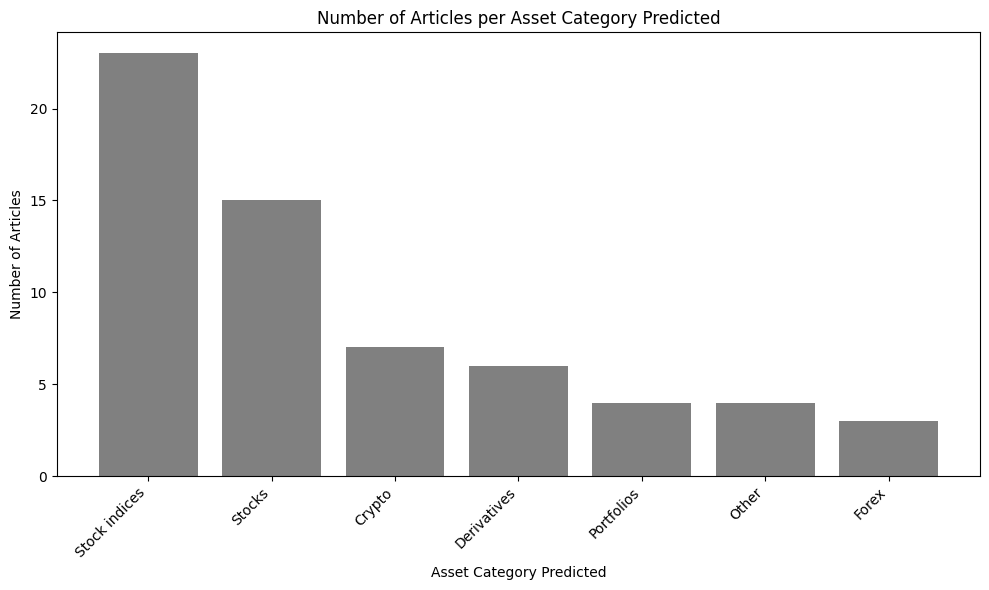
\includegraphics[width=1\linewidth]{Images/articles_per_asset_type_predicted.png}
    \caption{Asset type predicted}
    \label{fig:asset_type_predicted}
\end{figure}
\makeatletter

%%%
%% Hva skal skrives om her?
%%
%% Kanskje:
%% - Hvilket problem prøver man å løse ved å predikere asseten?
%% - Hvorfor er usikkerhetsestimater nyttige i denne konteksten?
%% - Hva har blitt gjort i artiklene i samplet?
%%
%% Bare se an hvor interessant det blir når vi har prøvd litt og så evt. flytte til descriptive statistics hvis det ikke er så interessant.
%%%



% --------- Stocks -------------------------------%
\subsubsection{Stocks}
Individual stocks are the most frequently analyzed asset class in the sample, with 25 articles. While a few studies focus on a single stock, the majority apply a common model to multiple stocks. Accurately predicting stock prices has proven challenging due to market efficiency \parencite{fama1970efficient}, which posits that prices fully incorporate all available information. In contrast, volatility has demonstrated greater  \parencite{poon2003forecasting}, emphasizing the relevance of uncertainty estimation for stocks. 

Most authors are motivated by the need for accurate forecasts of individual stock fluctuations to inform investor decisions and develop trading strategies. Trading strategies rely on informed beliefs about future price movements \parencite{vuletic2024finGAN}, and accurate range predictions are valuable for risk management \parencite{Li2024DeepAR}, as improved uncertainty estimates can help investors make more informed decisions regarding individual stocks and optimize profits. As \textcite{govindasamy2014prediction} note, the main problem faced by investors is that they do not have a clear idea on what stocks to invest in to maximize profits.  

Some studies do however study how external factors impact the uncertainty of individual stocks across countries and sectors differently \parencite{chandra2021bayesian, soleymani2022longterm}. Notably, \textcite{chandra2021bayesian} select stocks from mutiple counties to analyze the COVID-19 pandemic effect on different individual stock's fluctuations, highlighting the varying impact global events on asset-level uncertainty and underscoring the need for robust uncertainty quantification. 

% --------- stock Indicies-------------------------%
\subsubsection{Stock indices}
Stock indices are the second most prevalent category in the sample with 20 articles, with American, European and Asian indices dominating. Since indices are typically composed by multiple stocks from different sectors, they are generally less volatile than individual stocks and more indicative of the general state of the economy \parencite{sezer2020financial}. Therefore, uncertainty quantification can provide valuable insight into underlying market volatility. 

While most authors are motivated by the trading purposes of accurately forecasting indices, given that they are among the most important assets in the financial market, any of those emphasizing uncertainty are motivated by underlying market investigation. \textcite{Suphawan2022gpr} point out that stock price indices reflect the market, and reliable uncertainty estimates are therefore valuable in financial decision-making and risk management \parencite{Wang2021gpr}. Furthermore, \textcite{Wang2021gprensemble} state that accurate forecasts of fluctuation characteristics of indices can help government departments to timely and effectively supervise and guide the market to avoid financial risk. In addition, with the globalization of the world economy, several studies are focused on the interdependencies between indices in different across the world \parencite{cao2019multi} \parencite{Malagrino2018Forecasting}, making uncertainty estimates important to support risk management strategies on international scale.

% --------- Portfolios --------------------------%
\subsubsection{Portfolios}
9 articles in the sample focus on portfolios, referring to articles where the authors explicitly construct combinations of assets and forecasts it's value, returns or assess risk measures. Across the studies, the primary motivation is to maximize portfolio returns while incorporating financial risk measures to assess and manage uncertainty. In addition, \textcite{Risk2018gpr} actualize regulatory compliance with Solvency II requirements in insurance for risk assessment at the 99.5\% confidence-level. \textcite{kim2023portfolio} highlight the motivation for using a probabilistic model as opposed to deterministic models due to distributional outputs, and as the variance of predicted distributions can signify uncertainty, the models maximizing returns and minimizing risk in parallel. Most studies derive quantile-based risk measures from distributional outputs, with \textcite{Fatouros2023DeepVaR, arian2022encoded, caprioli2023quantifying} focusing on VaR, and  \textcite{Risk2018gpr, Min2023BlackLitterman} extend use to TVaR and CVaR respectfully. 

% --------- Crypto -----------------------------%
\subsubsection{Crypto}
There are 5 articles in the sample focused on forecasting cryptocurrencies, with Bitcoin being the most prevalent subject. Cryptocurrency markets are known for high volatility and fluctuating dynamics, posing significant challenge for accurate point predictions making uncertainty quantification especially relevant for risk-aware trading. Recent studies of the most frequently traded cryptocurrencies suggest that the markets are becoming increasingly efficient and intereconncted, although efficiency and volatility fluctuate significantly over time \parencite{noda2021evolution, liu2019volatility, gupta2022empirical}. This evolving efficiency makes the integration of cryptocurrencies into investment portfolios more attractive to investors.

Despite increasing efficiency, most articles in the sample are motivated by the fluctuating volatility and its implications for risk management. \textcite{Golnari2024Cryptocurrency} note that rapid value fluctuations make accurate prediction challenging and emphasize that understanding the inherent uncertainty in predictions and price dynamics is crucial for effective risk management in investment and trading. Similarly, 
\textcite{Almeida2024RiskForecasting} highlight the substantial loss potential in crypto markets, underscoring the paramount importance of understanding risk and implementing effective risk management strategies. \textcite{cocco2021predictions} state that the high volatility of cryptocurrencies, has made trading highly relevant in recent years, suggesting speculation may be profitable. 


% --------- Forex -----------------------------%
\subsubsection{Forex}
% Liquid market driven by many macroecomonic factors. Prob.AI applied to capture exchange rate flutions and uncertainty from complex international dynamic... essetion for both long and short term currency risk mangement
% Use forex volatility as external input to stock forecasting .. 
Foreign exchange (Forex) are one of the most liquid and interconnected asset class globally. The market is driven by several macroeconomic factors, geopolitical dynamics and international trading making uncertainty quantification essential for short and long term risk management and trade decisions. [KILDE]
In the sample, six articles address forex forecasting. They usually predict forex as part of several different application scenarios for testing their model, often motivated by inter-market dependencies, rater than uncertainty in the forex market alone. 
\textcite{li2010stochastic} argue that vagueness and uncertainty often present in certain data cannot effectively be managed by traditional models and necessitates probabilistic models to handled the forecasting challenges and integrate uncertainty in predictions \parencite{Moller2007Uncertainty, li2010stochastic}. 
\textcite{cao2019multi} highlight that understanding cross-market influences, like those between forex is essential for international risk management, where uncertainty estimates help to understand forex response to global market dynamics.  

\cite{Papaioannou2022gpr, Platanios2014gpr, 
tang2024period} all emphasize the importance of uncertainty estimates in financial market forecasting, motivated by the complex, high-volatility nature of the markets like forex markets. Their studies are motivated by making forecasting under unpredictability better and improve risk management ability to take informed decisions in interconnected markets.  


% --------- Derivatives -----------------------%
\subsubsection{Derivatives}
Nine articles in the sample focus on derivatives, which in this context are financial instruments whose value are derived from the underlying asset, such as stocks, bonds or indices. 

The most frequent derivative among the articles are volatility indices. \textcite{hortua2024forecasting, Daniali2021} analyze the VIX, while \textcite{Tian2023} extend their analysis to include the COEVI and TYVIX. Volatility indices, and the VIX in particular, are recognized as good indicators of investor sentiment and market turbulence, making it valuable for asset managers and regulators to foresee, but it remains difficult to forecast \parencite{hortua2024forecasting}. Probabilistic forecasts  of these indices could therefore be valuable to quantify the uncertainty around future volatility.

Options are another commonly derivative, with studies such as \textcite{Park2014gpr} focusing on KOSPI options, \textcite{DeSpiegeleer2018gpr} S\&P options and \textcite{tang2024period} different ETF options. \textcite{Park2014gpr} highlight a key limitation of traditional models like Black-Scholes: their inability to provide predictive distributions of the option prices. Probabilistic models, such as the GPR employed in their study, address this gap by offering predictions with uncertainty improving risk assessment - a primary motivation for the authors. 

Lastly, the sample include studies on credit default swap spreads \parencite{Law2017Practical} and capped volatility swaps \parencite{Hocht2024gpr}. 


\subsubsection{Commodities}
There are six articles in the sample that predict commodities, either gold or oil price, or commodity futures based on the exclusion criteria outlined in Section \ref{sec:methodology}. 

\textcite{Ahmed2023Enhancing} predict crude oil price with the aim to support strategic decision-making in energy investment. The motivation for using uncertainty estimates is crude oil's volatile price fluctuations which the authors claim to have an effect on stock of of renewable energy companies, therefore important to asses risk in investment timing and make informed decisions in the energy sector in unpredictable market conditions. 

\textcite{Wang2024GoldForecasting} is motivated by developing a probabilistic forecasting framework for gold prices to golds market dynamics. The authors point out golds important position in the global economy, both as a physical commodity and as a financial asset that has significant macroeconomic influence \parencite{Wang2024GoldForecasting, Pierdzioch2014Efficiency, Pierdzioch2014International}, and that gold cannot be effectivity foretasted using point estimates with reliable and credible forecasts, in particular in situation with extreme uncertainty \parencite{Wang2024GoldForecasting, Li2012Quantile}. Similar motivation can be seen in \textcite{Law2017Practical} where they predict commodity futures of gold and crude oil, and \textcite{Guo2022Risk} prediction crude oil futures.  

In the paper by \textcite{li2020multivariate}, where they predict agriculture future price, they highlights the importance of accurate forecast in order to reduce market uncertainty and support decision making in agriculture risk management and crop insurance programs, and being vital for policymakers and investors \parencite{li2020multivariate, Wang2017Performance, Ouyang2019Agricultural}. They also note that traditional models often assume independent variables and normal distribution but underscores that this assumption do not align with the real market conditions for commodities. 

\textcite{Guo2022} created interval predictions for non-ferrous metal futures. The authors highlights the economic importance of good uncertainty estimates due to the volatility of non-ferrous metal futures, which unpredictable price patters impact stocks, metal mining firms and futures investors \parencite{Guo2022, Zhang2022, Shao2016Productivity}. They are motivated by exploring a probabilistic model as they claim traditional models are not able to adequately capture these assets non-linear and non-stationary characteristic, which shows the need for more advance methods and interval predictions. 




% --------- Conclusion -----------------------%


% Write that we dont assess bonds.  

\subsubsection{Conclusion} % deside if we need this
Table \ref{table:conclusions_by_asset_classes} provides a summary of the primary focus and motivations of the authors making uncertainty estimates for the studied asset classes.

\begin{table}[H]
    \centering
    \caption[Summarizing conclusions by asset classes]{Summarizing conclusions by asset classes}
    \label{table:conclusions_by_asset_classes}
    \small
    \begin{adjustbox}{width=0.5\textwidth,center}
    \begin{tabular}{p{0.1\textwidth}p{0.40\textwidth}}
        \toprule
        \textbf{Asset Class} & \textbf{Conclusion} \\
        \midrule
        Stocks & \smallbullet{Enhance distributional stock forecasts for better trading and risk management} \smallbullet{Quantify how external factors impact stock uncertainty across markets} \\
        \addlinespace
        \hdashline[0.2pt/3pt]
        \addlinespace
        Stock indices & \smallbullet{Index uncertainty can reflects broader market volatility, aiding in financial decision-making} \smallbullet{Understanding interdependencies between international indices to enhance cross-border risk management} \\
        \addlinespace
        \hdashline[0.2pt/3pt]
        \addlinespace
        Portfolios & \smallbullet{Maximizing portfolio returns while leveraging uncertainty estimates for risk management} \smallbullet{Probabilistic models offer distributional outputs that support risk measures like VaR} \\
        \addlinespace
        \hdashline[0.2pt/3pt]
        \addlinespace
        Crypto & \smallbullet{High volatility of cryptocurrencies emphasize uncertainty quantification for risk-aware trading and investment} \smallbullet{Understanding fluctuating market dynamics for managing potential losses and leverage speculative opportunities} \\
        \addlinespace
        \hdashline[0.2pt/3pt]
        \addlinespace
        Forex & \smallbullet{Highly liquid and interconnected asset global driven by multiple factors making uncertainty quantification important for short- and long-term risk and trade management} \smallbullet{Cross-market dependencies necessitate probabilistic models for enhanced uncertainty estimation} \\
        \addlinespace
        \hdashline[0.2pt/3pt]
        \addlinespace
        Derivatives & \smallbullet{Probabilistic models address limitations of traditional methods  providing predictive distributions} \smallbullet{Volatility indices and option studies most prevalent} \\
        \addlinespace
        \hdashline[0.2pt/3pt]
        \addlinespace
        Commodities & \smallbullet{Uncertainty estimation important for strategic decisions making in i.e energy investment and agriculture risk management and policymakers} \smallbullet{Probabilistic models improve forecasting accuracy for commodities with non-stationary and non-linear characteristics} \\
        \addlinespace
        \addlinespace
        \bottomrule
    \end{tabular}
    \end{adjustbox}
\end{table}



%----------------------------------------------------%
% --------- Analysis by Type of Uncertainty-----------%
%----------------------------------------------------%

%Remember to include somehow the measures/how autors assess their uncertainty estimate - we also need to evaulate the strenght of these estimates, but that might be conclusion %


\subsection{Analysis by Type of Uncertainty}
\label{sec:analysis_by_type_of_uncertainty}
All the proposed models in our sample can provide estimates with some form of quantified uncertainty. However, the type of uncertainty and how the authors interpret it vary significantly. As shown in Figure \ref{fig:uncertainty_quantification_by_type_and_assessment}, many authors neither use nor interpret the uncertainty estimates at all. When they do present uncertainty estimates, they usually treat them as total uncertainty, without assessing whether it arises from modeling limitations (epistemic uncertainty) or from the inherent volatility of the underlying asset (aleatoric uncertainty). This distinction is crucial for investment decisions because it's important to know whether the uncertainty is due to an unreliable model or a risky asset.

Furthermore, only a minority of articles evaluate the quality and usefulness of the uncertainty estimates, and even fewer compare these estimates against traditional models. The following sections explore the various ways uncertainty quantification has been used in the sample articles, the financial relevance of each type of uncertainty, and how different uncertainty estimates have been and can be assessed. Summarizing results and conclusions by type of uncertainty are shown in Table \ref{table:conclusions_by_uncertainty}.


\begin{figure}[H]
    \centering
    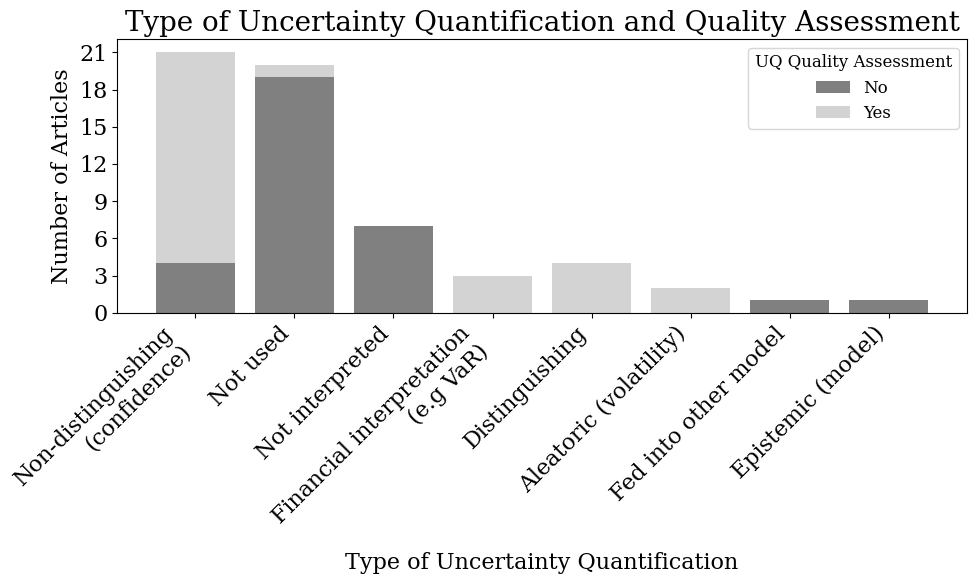
\includegraphics[width=1\linewidth]{Images/uncertainty_quantification_by_type_and_assessment.png}
    \caption{How the authors have interpreted the uncertainty estimates from the models and whether they have assessed the accuracy/quality of the estimates}
    \label{fig:uncertainty_quantification_by_type_and_assessment}
\end{figure}


%--------------------Not Interpreted or not used-------------------------%
\subsubsection{Not used}

Among the 62 articles in the sample, [19] do not in any way mention or illustrate that their models can produce outputs with uncertainty, even though they are utilizing models that inherently have the capability. Instead, they leverage probabilistic frameworks attempting to produce better point estimates. For most authors the motivation for using a probabilistic models nevertheless is pre-discovered accuracy in point predictions, e.g. \parencite{jang2018generative,Park2014gpr}, pre-processing or optimization e.g. \parencite{li2020multivariate, choudhury2020enhancing} or for better generalization e.g. \parencite{Papaioannou2022gpr,Thawornwong2004pnn}.

\subsubsection{Not interpreted}

In 7 articles, the probabilistic outputs from the model are presented, but not interpreted or assigned any financial or technical meaning. Generally, this is simply due to a non-existing focus on uncertainty estimation, but rather accuracy of point predictions \parencite{DeSpiegeleer2018gpr} or accuracy of category classifications e.g. \parencite{Malagrino2018Forecasting, Zhang2016}


%-----------------------Epistemic-----------------------------%
\subsubsection{Epistemic (model-uncertainty)}
Epistemic uncertainty arises from uncertainty about which model or set of weights is correct.

Only one article in the sample \parencite{hassan2023} interprets the quantified uncertainty as purely epistemic. Hassan proposes a Bayesian LSTM model tasked with predicting the price of Bitcoin. Specifically, Monte Carlo dropout is used to estimate the LSTM weights—a Bayesian inference technique introduced by \textcite{gal_ghahramani_2015}. This technique involves keeping dropout active during prediction time, allowing the model to generate as many predictions as desired. These predictions form a distribution that captures the model's uncertainty about which weights are optimal. This technique is not able to capture the latent volatility and provide a total uncertainty estimate, but the author does not claim that it does either.

[.. nevne noe om hvordan man kunne vurdert kvaliteten på epistemiske usikkerhetsestimater? f.eks. coverage probability ..]


%-------------------Aleatoric-------------------------------%
\subsubsection{Aleatoric (volatility)}
There are five articles in the sample that quantify uncertainty and interprets it as being aleatoric uncertainty, meaning the underlying data uncertainty, which in finance is referred to as the latent volatility.

[her kan vi nevne hva alle gjør tenker jeg, siden det er så få og såpass relevant]

[skrive her om at man kan bruke disse estimatene til å regne ut financial risk measures]

[skrive om hvordan man kan assesse aleatoric uncertainty-estimater og hvordan de har gjort det]

%-----------------------Total uncertainty--------------------------%

\subsubsection{Total uncertainty (non-distinguishing)}
Out of the 38 articles where the authors interpret uncertainty, the majority (20) treat it as total uncertainty. In this context, the uncertainty is supposed to indicate how likely it is that the prediction is accurate. However, they do not identify the sources of uncertainty—epistemic and aleatoric—and it remains unclear how much uncertainty comes from each source. The authors often state that knowing the model's confidence in its predictions is useful in investment decisions. However, not distinguishing between aleatoric and epistemic uncertainty limits the models' usefulness in investment decisions because investors cannot determine whether the uncertainty in the predictions stems from the inherent riskiness of the underlying assets or from a poor model fit.

Additionally, many authors use uncertainty quantification techniques that are unsuitable for determining total uncertainty. For example, six articles in this category employ probabilistic AI models based on Bayesian methods. This approach is debatable because, in Bayesian models, uncertainty is inherently tied to the model's specification rather than the data itself. For instance, Bayesian neural networks treat the network weights as random variables, so any prediction uncertainty arises directly from the uncertainty in these weights. Consequently, Bayesian techniques have limited usefulness for quantifying uncertainty in financial time series as they ignore the existence of a latent volatility that changes over time [trengs kilder for å støtte opp om dette?].

[hvis vi får til data på faculty, legge inn at mangel på distinksjon kanskje skyldes mangel på kompetanse i finans]

[skrive om hvordan man kan assesse total uncertainty-estimater og hvordan de har gjort det]

\subsubsection{Both epistemic and aleatoric uncertainty}

Only five articles estimate both epistemic and aleatoric uncertainty and distinguishes between the two.

[dette er også såpass sentralt at vi kanskje kan nevne kort hva som er approachen i hver av de fem artiklene?]

[skrive om hvordan man kan assesse denne typen estimater og hvordan de har gjort det]

\subsubsection{Fed into other model}

In three of the articles, the probabilistic output from the probabilistic AI model is not presented or interpreted directly, but is used as input to another model. [.. her kan vi kanskje nevne eksempler ..]

\begin{figure}[H]
    \centering
    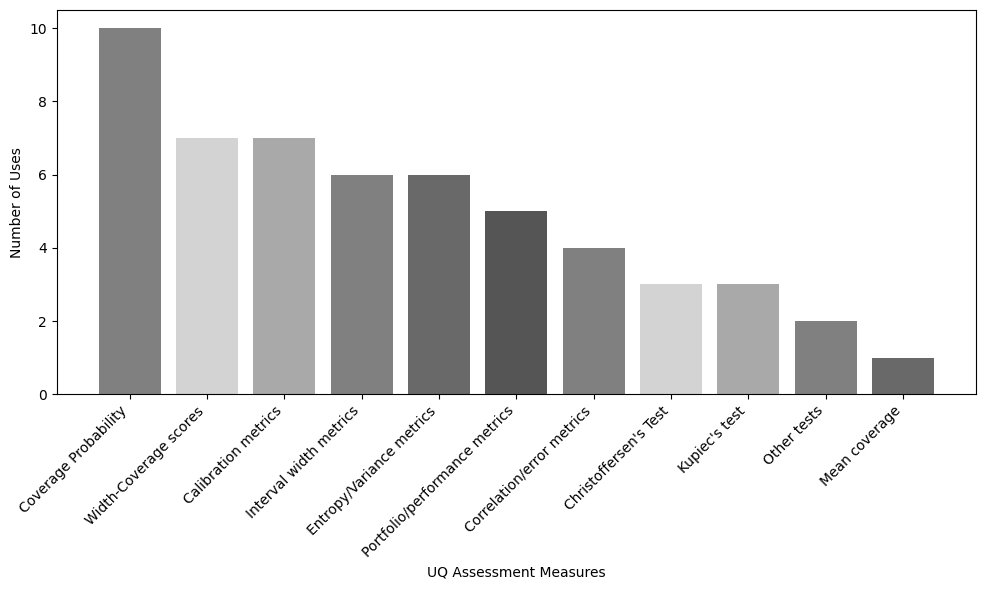
\includegraphics[width=1\linewidth]{Images/UQ assesment measures.png}
    \caption{UQ Assessment Measures}
    \label{fig:assesment_measures}
\end{figure}

%----------------------Conclusion----------------------------%

\subsubsection{Conclusion} % deside if we need this
\begin{table}[H]
    \centering
    \caption[Summarizing conclusions by type of uncertainty]{Summarizing conclusions by type of uncertainty}
    \label{table:conclusions_by_uncertainty}
    \small
    \begin{adjustbox}{width=0.5\textwidth,center}
    \begin{tabular}{p{0.1\textwidth}p{0.40\textwidth}}
        \toprule
        \textbf{Type of Uncertainty} & \textbf{Conclusion} \\
        \midrule
        Not used & \smallbullet{Point 1} \smallbullet{Point 2}  \\
        \addlinespace
        \hdashline[0.2pt/3pt]
        \addlinespace
        Not interpreted & \smallbullet{Point 1} \smallbullet{Point 2}  \\
        \addlinespace
        \hdashline[0.2pt/3pt]
        \addlinespace
        Epistemic (model-uncertainty) & \smallbullet{Point 1} \smallbullet{Point 2}  \\
        \addlinespace
        \hdashline[0.2pt/3pt]
        \addlinespace
        Aleatoric (volatility) & \smallbullet{Point 1} \smallbullet{Point 2}  \\
        \addlinespace
        \hdashline[0.2pt/3pt]
        \addlinespace
        Total uncertainty (non-distinguishing) & \smallbullet{Point 1} \smallbullet{Point 2}  \\
        \addlinespace
        \hdashline[0.2pt/3pt]
        \addlinespace
        Both epistemic and aleatoric uncertainty & \smallbullet{Point 1} \smallbullet{Point 2}  \\
        \addlinespace
        \hdashline[0.2pt/3pt]
        \addlinespace
        Fed into other model & \smallbullet{Point 1} \smallbullet{Point 2}  \\
        \addlinespace
        \addlinespace
        \bottomrule
    \end{tabular}
    \end{adjustbox}
\end{table}

% ---------------------------------------------------------------%
% --------------------------Discussion --------------------------%
% ---------------------------------------------------------------%


\subsection{Discussion}
\label{sec:discussion}
This section will analyze the results in relation to each of the research questions presented in Section \ref{sec:introduction}.
% go through each reserach question and answer explicitly




\textbf{Summarize to what extent and in what way existing research are using uncertainty estimates from probabilistic AI models as a measure of volatility, model uncertainty or financial risk measures for financial time series}
\\ % Write here

Throughout this review we have seen how existing research frequently employ various probabilistic AI models to forecast financial time series, with frequently employed models discussed in section \ref{sec:analysis_by_model} being Bayesian Neural Networks (BNNs), Gaussian Regression Processes (GPRs) and probabilistic Recurrent Neural Network (RNN) extension. The primary focus of existing research seems to concern improving point prediction accuracy for different assets, and that potential for uncertainty estimation is underutilized. Out of the [64] articles reviewed, only [XX] make a meaningful interpretation of uncertainty estimates generated by their models, only [XX] of these explicitly assess the quality of their estimates, while [XX] studies do not use or interpret uncertainty estimates at all. 

 - 2. Measure of volatility: (aleatoric uncertainty), how many do it, what models are they using, of those predicting the VIX what do they do?, 

 3. Model uncertainty (epistemic): very few do it, what models do they use, and why do people not do it? - because they just don't distinguish and just interpret model uncertainty as total. What models can inherently do it, and can be a area for future research?

 4. Financial risk measures: how many do it, what models are promising, what, Christoffersen's test or other adequacy metrics are underutilized, with only X studies rigorously validating their risk measures with adequacy and accuracy. 

 5. Inadequate benchmarking: often outperform in point-predictions, but generally lack good/standardized testing validation for uncertainty estimates. Standardized benchmarks or frameworks could help quantify true value of the estimates in a financial context. 


\textbf{Analyze researchers' motivation for making predictions with uncertainty and how it differs for different asset classes}
\\ % Write here
A primary motivation for authors utilizing probabilistic models across asset classes is to estimate uncertainty without having to assume any underlying distribution of data when employing non-parametric models. Traditional models usually rely on normality assumptions, a suboptimal restriction given the documented deviations of financial data from normal distribution. Additionally, several researchers highlight the self-learning and noise-tolerant capabilities of probabilistic and machine learning models.

The motivations for making predictions with uncertainty estimates also vary among the asset classes, and are primarily influenced by the unique market characteristics and investor needs inherent in each class. For assets known to have high volatility, like individual stocks or cryptocurrencies, the authors seem motivated mainly by the need to manage risk for investors and enhancing trading strategies. The frequent price fluctuations of these assets underscore the importance of accurate uncertainty estimation, both to inform investment decisions and mitigate potential losses or facilitate speculation, a main motivational factors of the authors. 

For stock indices, researches still seem primarily motivated by risk management considerations for investment and trading. However, given that some indices like the S\&P 500 closely represent overall market performance and conditions, some researches extend their motivations beyond this perspective to encompass a broader understanding of market volatility. This include uncertainty estimation for insights into systematic risk and market dynamics. Additionally, in Forex and large international indices, some researches seem motivated by the understanding global interconnection and cross-market influences through uncertainty estimations.

For the researchers assessing portfolios, the primary motivation lies in  the need for uncertainty estimations for financial risk measures and regulatory compliance. Most studies construct measures like VaR, utilizing distributional output from the probabilistic models in attempt to provide more accurate risk assessment of portfolios.

\textbf{Compare the promise of these models compared to other machine learning models and traditional econometric models in uncertainty estimation}
% Write here

There are only 6 models in the sample where created uncertainty estimates are benchmarked against traditional models. In 5 of these articles authors benchmark against GARCH variants, and only in 2 cases does the proposed model clearly outperform the traditional one. These models are the DeepVaR proposed by \textcite{Fatouros2023DeepVaR} and the GPMCH by \textcite{Platanios2014gpr}. However, there are 11 articles in which the authors compare the uncertainty estimate of their model with another machine learning model, where only 1 also compare against a traditional econometric model. All models outperform the machine learning model benchmark. These findings suggest lacking and unsatisfactory benchmarking against traditional econometric like GARCH, making it difficult to draw definitive conclusions.

When it comes to point predictions there are 26 articles where the researchers benchmark their points predictions against traditional models. Of these, 17 show clear superior performance, demonstrating promise in accurate predictive power. A total of 45 articles benchmark their model against other machine learning models, and a 37 of them outperform their benchmarks. Once again, this suggest a bias towards comparing with other machine learning models rather then traditional econometric models. Even though these results demonstrate promising accuracy for point predictions for probabilistic models, there is strong evidence of publishing bias in finance, making it difficult to conclude on the soundness of these results \parencite{Kim2015SignificanceTI}.

In conclusion, probabilistic models seem to provide improved point predictions and have interesting properties for financial modeling, such as being able to estimate non-parametric distributions and capturing non-linear patterns. There are some models demonstrating promising results in uncertainty estimation, but limited benchmarking especially with traditional models makes it difficult to conclude on the real promise of the models.


\textbf{Can probabilistic models provide an improved understanding of risk and volatility compared to econometric models}
\\ % Write here
- It is well known that distributions of asset returns have fatter tails than the normal distribution [kilde] which makes probabilistic AI models ability to estimate non parametric distributions interesting

- As an investor it is important and valuable to know where the uncertainty is coming from, something probabilistic models may provide better compared to traditional econometric models 

- maybe say something about epistemic and aleatoric uncertainty in this part

\textbf{Which metrics are used for assessing probabilistic AI models and what is the most appropriate metric for assessing the quality of the produced uncertainty estimates?}
\\ % Write here

People use this and this and that. (Coverage, calibration, width, interval score). However, many articles fail to test the significance of their uncertainty estimates using significance tests such as ... 
Generally a standardized testing procedure is lacking both in common model benchmarks, but also in the tests performed. 
 
 
 - Perhaps propose a Christoffersen's testing framework here, with accuracy measures as a second step: To conclusively say that an AI model for volatility is useful it must pass something like Christoffersen’s test, and it must outperform e.g. GARCH in terms of coverage relative to interval width (resolution vs. reliability or whatever you want to call it) OR some scoring/accuracy function

 [tenker key takeaway i denne seksjonen bør være at man må teste at modellen gir riktig unconditional coverage og at violations er independent over tid, aka. christoffersen's test, og at man også må bruke scoring funksjoner som kan vise at estimatene man produserer er bedre enn tradisjonelle modeller, f.eks. coverage probability ifht. intervallbredde. mangler man et av disse punktene er det umulig å si om modellen har noe for seg.]

\textbf{How do probabilistic AI models integrate with financial risk measures such as Value at Risk (VaR) and Expected Shortfall (ES)?}
% Write here

There are 8 articles in total creating financial risk measures using probabilistic models, where tail-risk estimates for portfolios such as VaR is the most prevalent. Several authors argue that traditional parametric methods for VaR estimation are limited by explicit return distribution and linear dependency assumptions, which necessarily do not hold for financial time series \parencite{arian2022encoded,Fatouros2023DeepVaR}. Probabilistic models like Variational Auto-Encoders (VAE) and DeepAR, utilized in several articles for VaR estimation, directly address this limitation by generating probabilistic forecasts of the entire return distribution without explicit parametric assumptions. The distributional output of the models can be used directly for tail-risk estimation. Probabilistic models therefore integrate well with financial risk measures such as VaR or ES, and can be used to effectively address limitations of traditional models. While achieved results vary compared to traditional models, largely due to partially insignificant estimates, further research on different non-parametric probabilistic models show promise to create more meaningful VaR estimates for financial risk management.

\textbf{Identity possible areas for further research}
% Write here

- testing different probabilistic models to create significant financial risk estimates such as VaR

her syns jeg vi burde komme med en del tydelige recommendations for fremtidig research:

1. man burde alltid skille mellom epistemic og aleatoric uncertainty når man modellerer finansielle tidsserier

2. dersom man lager en modell der usikkerhet er i fokus er det kritisk at de aleatoriske usikkerhetsestimatene testes rigorously, med f.eks. en kombinasjon av christoffersen's test og scoring-funksjoner der man sammenligner med andre modeller

3. hvis det ikke finnes allerede burde noen lage et tydelig rammeverk for hvordan man tester fulle distribusjoner, altså ikke bare f.eks. 95\% VaR men hver eneste kvantil

4. det er veldig få artikler hvor ai-modellers evne til å produsere ikke-parametriske distribusjoner utnyttes fullt ut, det hadde vært interessant om det ble gjort i større grad og om det ble testet ordentlig

5. Combine probabilistic AI models with traditional models like GARCH to estimate the uncertainty, where few articles propose such a hybrid model